% Options for packages loaded elsewhere
\PassOptionsToPackage{unicode}{hyperref}
\PassOptionsToPackage{hyphens}{url}
%
\documentclass[
]{book}
\usepackage{lmodern}
\usepackage{amsmath}
\usepackage{ifxetex,ifluatex}
\ifnum 0\ifxetex 1\fi\ifluatex 1\fi=0 % if pdftex
  \usepackage[T1]{fontenc}
  \usepackage[utf8]{inputenc}
  \usepackage{textcomp} % provide euro and other symbols
  \usepackage{amssymb}
\else % if luatex or xetex
  \usepackage{unicode-math}
  \defaultfontfeatures{Scale=MatchLowercase}
  \defaultfontfeatures[\rmfamily]{Ligatures=TeX,Scale=1}
\fi
% Use upquote if available, for straight quotes in verbatim environments
\IfFileExists{upquote.sty}{\usepackage{upquote}}{}
\IfFileExists{microtype.sty}{% use microtype if available
  \usepackage[]{microtype}
  \UseMicrotypeSet[protrusion]{basicmath} % disable protrusion for tt fonts
}{}
\makeatletter
\@ifundefined{KOMAClassName}{% if non-KOMA class
  \IfFileExists{parskip.sty}{%
    \usepackage{parskip}
  }{% else
    \setlength{\parindent}{0pt}
    \setlength{\parskip}{6pt plus 2pt minus 1pt}}
}{% if KOMA class
  \KOMAoptions{parskip=half}}
\makeatother
\usepackage{xcolor}
\IfFileExists{xurl.sty}{\usepackage{xurl}}{} % add URL line breaks if available
\IfFileExists{bookmark.sty}{\usepackage{bookmark}}{\usepackage{hyperref}}
\hypersetup{
  pdftitle={Documento Técnico N°3: Registros Administrativos},
  pdfauthor={Dirección Nacional de Mercados y Estadísticas - Subsecretaría de Desarrollo Estratégico},
  hidelinks,
  pdfcreator={LaTeX via pandoc}}
\urlstyle{same} % disable monospaced font for URLs
\usepackage{longtable,booktabs}
\usepackage{calc} % for calculating minipage widths
% Correct order of tables after \paragraph or \subparagraph
\usepackage{etoolbox}
\makeatletter
\patchcmd\longtable{\par}{\if@noskipsec\mbox{}\fi\par}{}{}
\makeatother
% Allow footnotes in longtable head/foot
\IfFileExists{footnotehyper.sty}{\usepackage{footnotehyper}}{\usepackage{footnote}}
\makesavenoteenv{longtable}
\usepackage{graphicx}
\makeatletter
\def\maxwidth{\ifdim\Gin@nat@width>\linewidth\linewidth\else\Gin@nat@width\fi}
\def\maxheight{\ifdim\Gin@nat@height>\textheight\textheight\else\Gin@nat@height\fi}
\makeatother
% Scale images if necessary, so that they will not overflow the page
% margins by default, and it is still possible to overwrite the defaults
% using explicit options in \includegraphics[width, height, ...]{}
\setkeys{Gin}{width=\maxwidth,height=\maxheight,keepaspectratio}
% Set default figure placement to htbp
\makeatletter
\def\fps@figure{htbp}
\makeatother
\setlength{\emergencystretch}{3em} % prevent overfull lines
\providecommand{\tightlist}{%
  \setlength{\itemsep}{0pt}\setlength{\parskip}{0pt}}
\setcounter{secnumdepth}{5}
%%% REFERENCIAS
        \usepackage{hyperref}
        % links del indice en negro; citas y URL en azul
        \hypersetup{colorlinks = true, urlcolor={blue}, 
        citecolor={blue}, linkcolor ={blue}}
\usepackage[spanish]{babel} % Idiomas en los que se escribe el documento. 
\usepackage{booktabs}
\usepackage{amsthm}

\usepackage[final]{pdfpages}

\makeatletter
\def\thm@space@setup{%
  \thm@preskip=8pt plus 2pt minus 4pt
  \thm@postskip=\thm@preskip
}
\makeatother
\let\oldmaketitle\maketitle
\AtBeginDocument{\let\maketitle\relax}
\ifluatex
  \usepackage{selnolig}  % disable illegal ligatures
\fi
\usepackage[]{natbib}
\bibliographystyle{apalike}

\title{Documento Técnico N°3: Registros Administrativos}
\usepackage{etoolbox}
\makeatletter
\providecommand{\subtitle}[1]{% add subtitle to \maketitle
  \apptocmd{\@title}{\par {\large #1 \par}}{}{}
}
\makeatother
\subtitle{Descripción, Análisis y Utilización de los Registros Administrativos para la medición del Turismo}
\author{Dirección Nacional de Mercados y Estadísticas - Subsecretaría de Desarrollo Estratégico}
\date{20 de septiembre de 2021}

\begin{document}
\maketitle

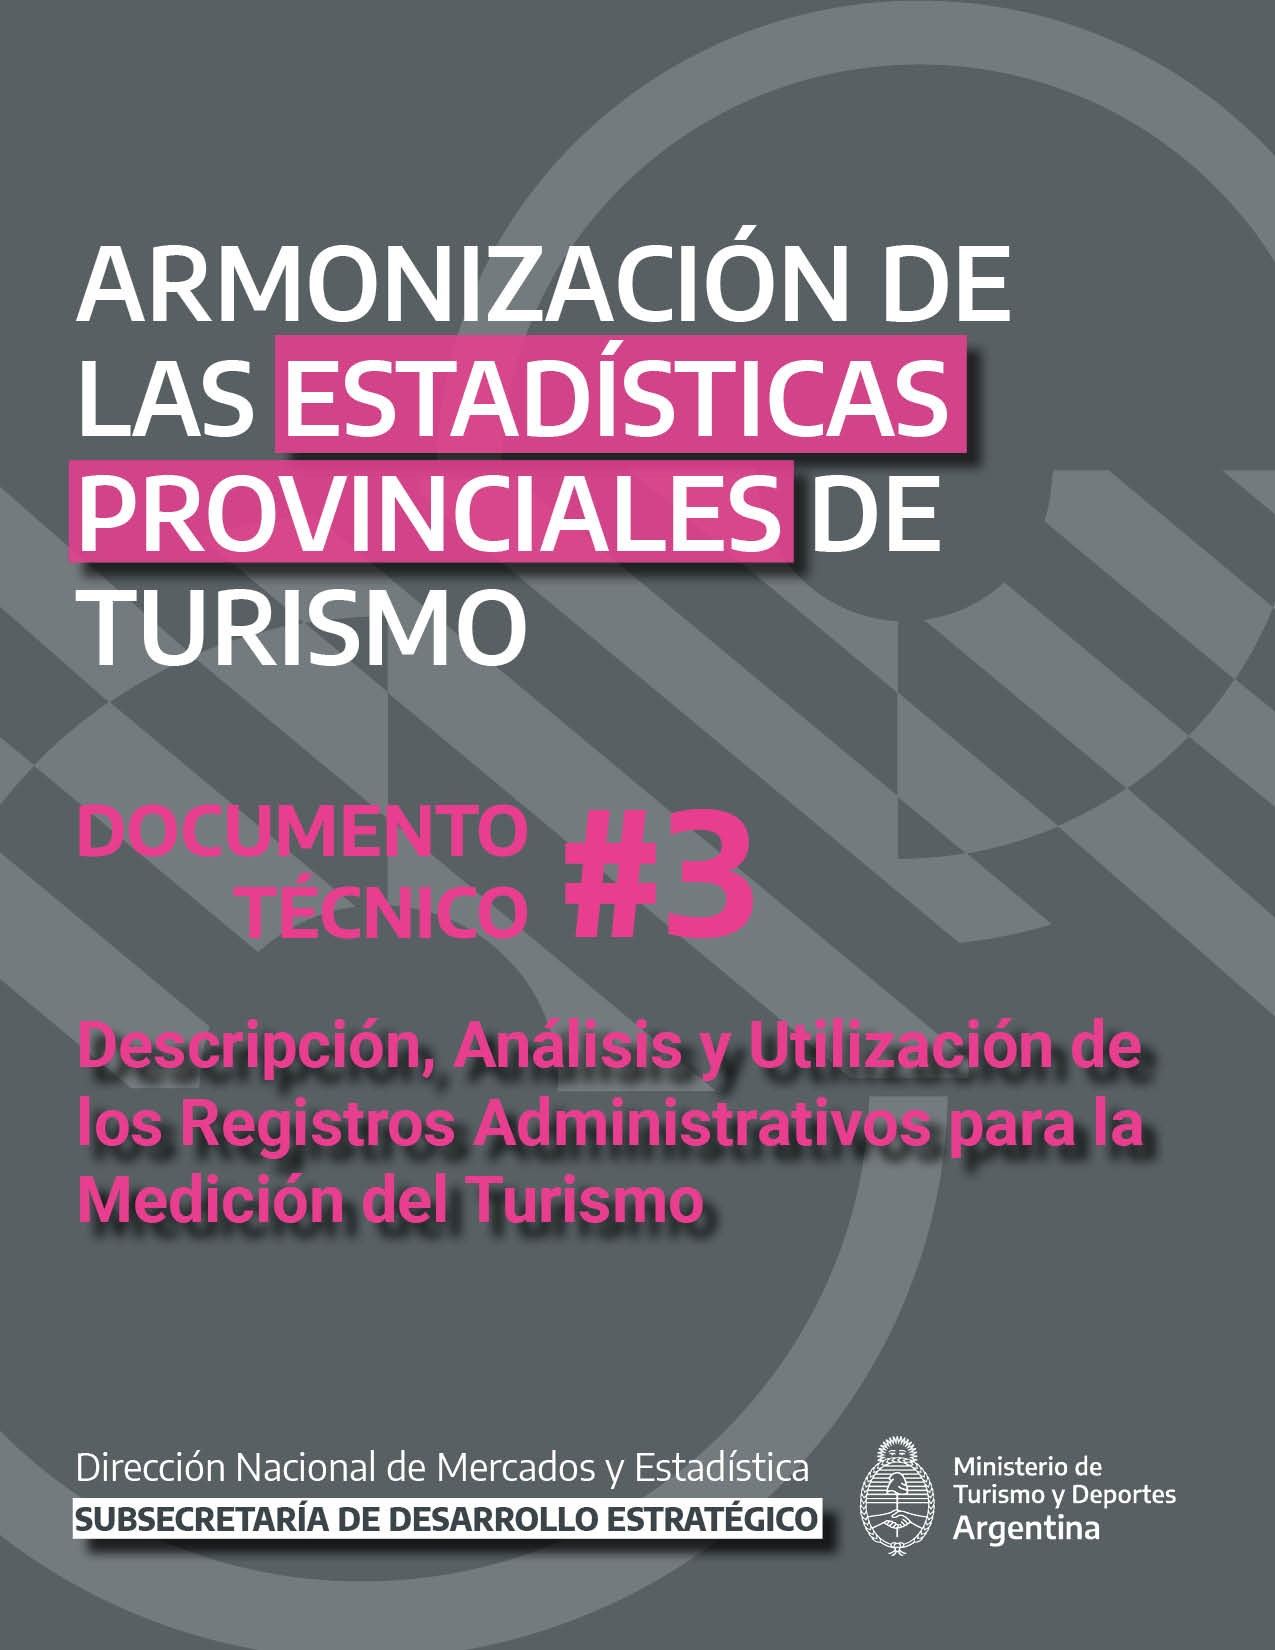
\includepdf[pages={1}, scale=1]{DT3Portada.pdf}
\newpage

\let\maketitle\oldmaketitle
\maketitle

{
\setcounter{tocdepth}{1}
\tableofcontents
}
\hypertarget{presentaciuxf3n}{%
\chapter*{Presentación}\label{presentaciuxf3n}}
\addcontentsline{toc}{chapter}{Presentación}

El presente documento, \textbf{Descripción, Análisis y Utilización de los Registros Administrativos para la medición del Turismo}, se enmarca en el proyecto de \href{https://armonizacion.yvera.tur.ar//}{Armonización de las Estadísticas de Turismo en las Provincias} de la \textbf{Dirección Nacional de Mercados y Estadísticas de la Subsecretaría de Desarrollo Estratégico del Ministerio de Turismo y Deportes}. El objetivo general de este proyecto es contribuir con propuestas metodológicas para los sistemas de estadísticas de turismo provinciales que orienten a producir indicadores provinciales básicos y comparables.

Además de este, se encuentran disponibles una serie de documentos técnicos que abordan otras problemáticas vinculadas a la producción de estadística de turismo:

\begin{itemize}
\item
  \href{https://dnme-minturdep.github.io/DT1_medicion_turismo/}{Documento Técnico \#1}: Conceptos y elementos básicos para la medición provincial de los turistas
\item
  \href{https://dnme-minturdep.github.io/DT2_encuestas/}{Documento Técnico \#2}: Propuestas Metodológicas para las encuestas de ocupación en alojamientos turísticos
\item
  \href{https://dnme-minturdep.github.io/DT4_perfiles/}{Documento Técnico \#4}: Propuestas Metodológicas para las Encuestas de Perfil del Visitante
\item
  \href{https://dnme-minturdep.github.io/DT5_actividad_empleo/}{Documento Técnico \#5}: Medición de la contribución económica del turismo: actividad y empleo
\end{itemize}

\hypertarget{documento-tuxe9cnico-nuxba3---resumen}{%
\subsection*{Documento Técnico Nº3 - Resumen}\label{documento-tuxe9cnico-nuxba3---resumen}}
\addcontentsline{toc}{subsection}{Documento Técnico Nº3 - Resumen}

Este documento presenta la problematización en torno a la utilización de los Registros Administrativos, como fuente secundaria de información para la elaboración de estadísticas tendientes a la medición del Turismo en las jurisdicciones provinciales y municipales del país. En este sentido, internacionalmente se ha remarcado la importancia que los mismos poseen:

\begin{quote}
``\ldots la experiencia confirma, la necesidad de promover el uso de fuentes administrativas asociadas a los controles en frontera y los flujos de transporte, entre otras razones, porque es imposible desarrollar un Sistema de Estadísticas de Turismo y las Cuentas Satélite basándose exclusivamente en encuestas\ldots{}'' \citep{ife2006}.
\end{quote}

En el \textbf{Capítulo} \ref{los-registros-administrativos} se realiza una síntesis introductoria teórica en torno a la conceptualización de los registros administrativos y, a la vez, se propone una secuencia de pasos para desarrollar y potenciar el aprovechamiento de los mismos.

En el \textbf{Capítulo} \ref{clasificaciones} se propone la clasificación de los registros administrativos en base a las distintas dimensiones vinculadas a la información proporcionada por los diferentes tipos de registros que se han sistematizado en el marco del Proyecto.

Finalmente, en el \textbf{Capítulo} \ref{algunos-ejemplos} se elabora un esquema de análisis para la comprensión conceptual de los posibles usos de los registros administrativos, con el propósito de brindar elementos para su interpretación y utilización como insumo para la producción de estadísticas de Turismo, reflexionando mediante ejemplos puntuales que sirven como disparadores para la innovación de metodologías que permitan realizar el proceso de conversión de los datos originales en información estadística.

\hypertarget{los-registros-administrativos}{%
\chapter{\texorpdfstring{\textbf{Los registros administrativos}}{Los registros administrativos}}\label{los-registros-administrativos}}

El objetivo de los apartados siguientes es abordar la importancia y la metodología de utilización de los Registros Administrativos como insumo clave para la elaboración de estadísticas de Turismo y, a la vez, proponer una reflexión respecto de los usos potenciales de los mismos.

\hypertarget{quuxe9-son}{%
\section{¿Qué son?}\label{quuxe9-son}}

En el marco de la generación de estadísticas básicas, una de las principales fuentes de información proviene de los registros administrativos (\texttt{RA}). Según la evidencia y las experiencias relevadas, actualmente es escasa su utilización como insumo para la elaboración y producción de estadísticas tendientes a la medición del Turismo.

La explotación de los RA se posiciona como una herramienta para la producción de estadísticas de Turismo a nivel nacional, provincial y/o departamental, ya que pueden complementarse con la información que surge de otras fuentes, por ejemplo, operativos propios (del organismo en cuestión) u otras fuentes secundarias.

En la literatura especializada no se encuentra una definición universal respecto de qué se entiende por registro administrativo. Pese a esto, resulta importante analizar algunas de las definiciones encontradas:

\begin{quote}
``\ldots todo registro resultante de necesidades fiscales, tributarias u otras, creado con la finalidad de viabilizar la administración de los programas de gobierno o para fiscalizar el cumplimento de obligaciones legales de la sociedad. Para su utilización con fines estadísticos es preciso evaluar su base conceptual y metodológica, clasificaciones, cobertura alcanzada, variables investigadas, calidad de las respuestas, procesamiento de los datos y frecuencia de disponibilidad de ellos\ldots{}'' \citep{cepal2003}.
\end{quote}

\begin{quote}
``\ldots aquellos registros de carácter administrativo y operativo, son procedimientos que utilizan las instituciones para registrar datos de las actividades propias de su función, muchas de ellas relacionadas con la oferta de un servicio público, otras que identifican a usuarios del Estado, y algunas que se derivan de las actividades realizadas con empresas e instituciones nacionales e internacionales, la cual no necesariamente coincide con los fines estadísticos, por lo que requiere un tratamiento especial para su utilización\ldots{}'' \citep{inei2004}.
\end{quote}

A partir de lo señalado anteriormente surge que el RA no es una fuente de origen estadístico propiamente dicho, ya que su finalidad es administrativa, y además, su propósito es servir para un control normativo. Es decir, registra un evento o acto individual referido a un individuo u objeto y lo afecta directamente.

Por ejemplo, en una operación de compra-venta de un objeto se emite una factura, lo que implica que se registra un evento normativo con fines fiscales; al solicitar un empleo se completa una planilla para evaluar el perfil del solicitante; al faltar una norma de tránsito se levanta una boleta de citación o una multa que deberá ser cancelada, etc. En conclusión, ninguno de estos eventos es propiamente estadístico, sin embargo, se convierte en una fuente de información estadística luego de ser tratada mediante procedimientos convenientes.

De manera genérica se plantea aquí la definición de los \texttt{RA} como:

\begin{quote}
``Aquella información que surge de los procedimientos administrativos y/o operativos que desarrollan y utilizan las instituciones (públicas o privadas) como método de registro de las diferentes actividades (turísticas y/o no turísticas) realizadas.''
\end{quote}

En base a las experiencias internacionales recopiladas, se da cuenta de los requerimientos que deben cumplir los procesos de diseño, recolección, producción y difusión de los \texttt{RA} \citep{dane2010a}. Éstos deben responder a criterios de calidad estadística, como lo son:

* \textbf{Credibilidad}: Se basa en la confianza que tienen los usuarios sobre el proceso estadístico del registro administrativo. Evalúa los «estándares estadísticos apropiados», es decir, políticas y prácticas objetivas para el diseño, recolección, almacenamiento, procesamiento y difusión de datos estadísticos \citep{ine2007}.

* \textbf{Oportunidad}, temporalidad y accesibilidad: Es el período en el que la información es de valor y se puede actuar o tomar decisiones acorde con ella. Estrechamente relacionada a la oportunidad está la puntualidad, que implica la existencia de una agenda de publicación y refleja el grado de cumplimiento de ella \citep{oecd2003}.

Según la Organización para la Cooperación y Desarrollo Económicos (OECD), la información estadística puede considerarse de calidad en la medida en que se encuentre disponible en el momento en que aún es relevante para el seguimiento y evaluación, y/o la toma de decisiones respecto al fenómeno que estudia o que es objeto de medición.

* \textbf{Accesibilidad}: Evalúa la rapidez de localización y el acceso dentro de la organización. La accesibilidad incluye la conveniencia de la manera en que los datos están disponibles, los medios de divulgación, la disponibilidad de metodologías, metadatos, datos y servicios de apoyo al usuario \citep{oecd2003}.

Es necesario tener en cuenta que la forma en que se presentan los datos a los usuarios sea clara y comprensible, lo que implica estrategias de difusión adecuadas e imparciales y si el usuario tiene acceso a metadatos actualizados, sin ningún tipo de restricción. Además, es necesario contar con sistemas de apoyo a los usuarios que utilizan los datos.

En términos de la CEPAL, este criterio contempla las \emph{«condiciones físicas en que los usuarios pueden obtener los datos: dónde y cómo pedirlos, tiempo de entrega, política clara de precios, formatos de disponibilidad, otros}»\citep{cepal2003}.

* \textbf{Pertinencia o relevancia}: Es una medida cualitativa del valor aportado por la información. El valor está directamente relacionado con el grado de utilidad para satisfacer el propósito por el cual la información fue buscada o solicitada. Depende de la cobertura de los tópicos requeridos y del apropiado uso de conceptos. La medición de la relevancia de un producto estadístico requiere de la identificación de su grupo de usuarios y sus necesidades \citep{oecd2003}. Los datos producidos por los \texttt{RA} tienen múltiples usos y usuarios que pueden cambiar con el tiempo.

Asimismo, cada uno de los múltiples \texttt{RA}, poseen características propias respecto de la forma en que se fueron sistematizando y registrando. En efecto, para su aprovechamiento como fuente secundaria para la producción de estadísticas metodológicamente elaboradas, resulta posible identificar diferentes aspectos respecto de la utilidad y los requerimientos que posean cada uno.

Entre los principales elementos respecto de la utilidad de los mismos, se puede destacar que:

\begin{enumerate}
\def\labelenumi{\roman{enumi})}
\item
  son una fuente de información importante y disponible;
\item
  pueden utilizarse como indicadores de evolución (aunque con ciertas limitaciones que se profundizan posteriormente en este documento), y a la vez, como insumos para la elaboración de estadísticas;
\item
  la obtención de dicha información posee bajo y/o nulo costo; por lo general;
\item
  cuentan con una alta cobertura y la información suministrada permite generar distintas desagregaciones, como por ejemplo, según niveles institucionales (provincial, departamental y/o municipal) y tipos de variables (sexo, edad, etc.).
\end{enumerate}

De manera complementaria, los requerimientos claves que se deberían contemplar para su utilización consisten en el análisis de las limitaciones de dicha fuente, ya que no cuentan con una metodología estadística que sistematice y recopile la información. Tanto para su utilización como insumo y/o para la elaboración de indicadores estadísticos se requiere, por lo general, un proceso de conversión que transforme las unidades administrativas en unidades estadísticas y, a la vez, en dicho proceso, se requiere diseñar y desarrollar una metodología con la secuencia lógica de diferentes pasos estadísticos.

En la figura que se presenta a continuación, se puede dar cuenta de las utilidades y los requerimientos que la utilización de los \texttt{RA} presenta.

\begin{figure}

{\centering 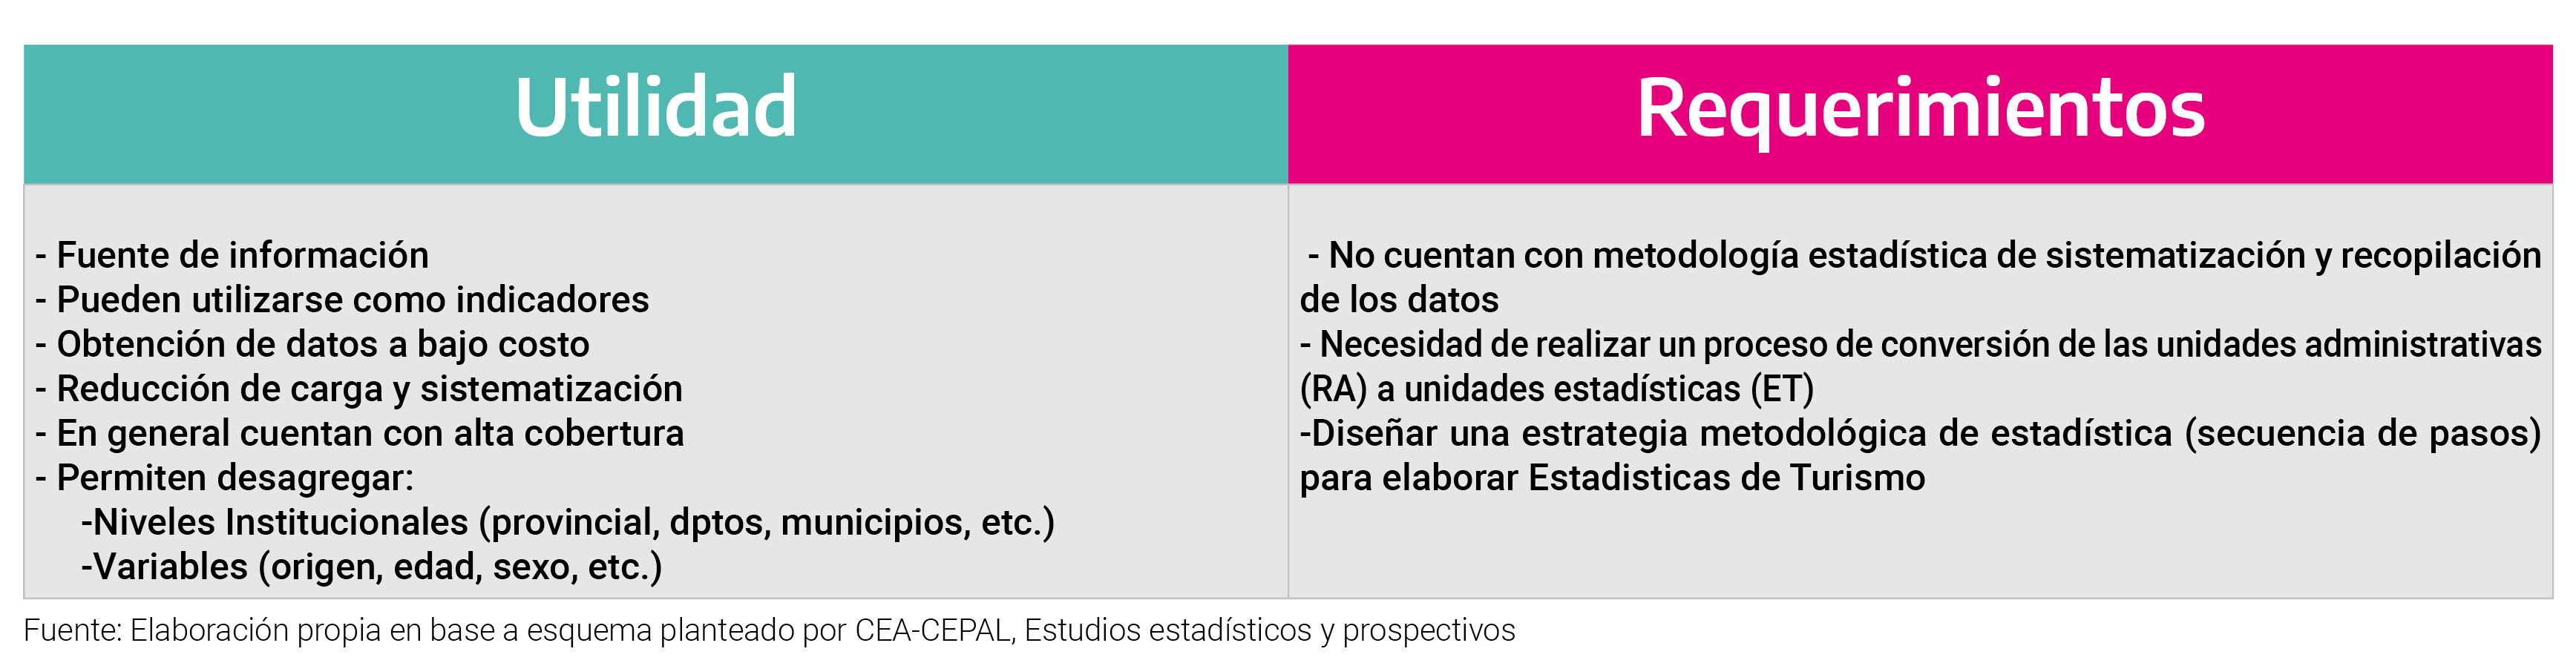
\includegraphics[width=1\linewidth]{imagenes/figura01} 

}

\caption{Utilidad y requerimientos para el uso de los Registros Administrativos}\label{fig:registrosadministrativos}
\end{figure}

El análisis que se haga de los datos generados a partir de los \texttt{RA} estará condicionado por la forma en que estas cuestiones sean encaradas y solucionadas tanto desde la propia institución que genera los datos como por el organismo que los utiliza con fines estadísticos. En efecto, se deben contemplar ciertos recaudos al momento de la utilización de los datos, la forma en que se los extrapole, los ponderadores que se utilicen, etc. con el propósito de procurar que las cifras obtenidas de las fuentes secundarias sean lo más representativas de la realidad que se procura captar.

El fortalecimiento de los \texttt{RA} para fines estadísticos constituye un proceso que busca desarrollar la base metodológica y conceptual, la oportunidad de recolección, las variables y la disponibilidad de la información recolectada, a través de una metodología que permita potencializarlos como fuente de información estadística para la toma de decisiones y la formulación de planes, proyectos y políticas públicas destinadas al sector turístico.

En este sentido, a fin de que un registro administrativo sea utilizado para un análisis estadístico se deberán contemplar, al menos, los siguientes criterios: la base metodológica, la clasificación con la que cuenta el registro, la cobertura geográfica, la calidad de la registración de los datos que posee, la temporalidad y oportunidad y los medios por los cuales se puede disponer de la información \citep{inegi2006}.

Como ya se ha mencionado, desarrollar una metodología válida y clara es fundamental para una correcta utilización de los RA en la confección de estadísticas del turismo (ET). Así, en la Figura N°1.2 se presenta un conjunto de etapas y/o fases para la correcta conversión de la información almacenada en los RA, tal que permitan abordar el objetivo buscado por quien los esté utilizando.

\begin{figure}

{\centering 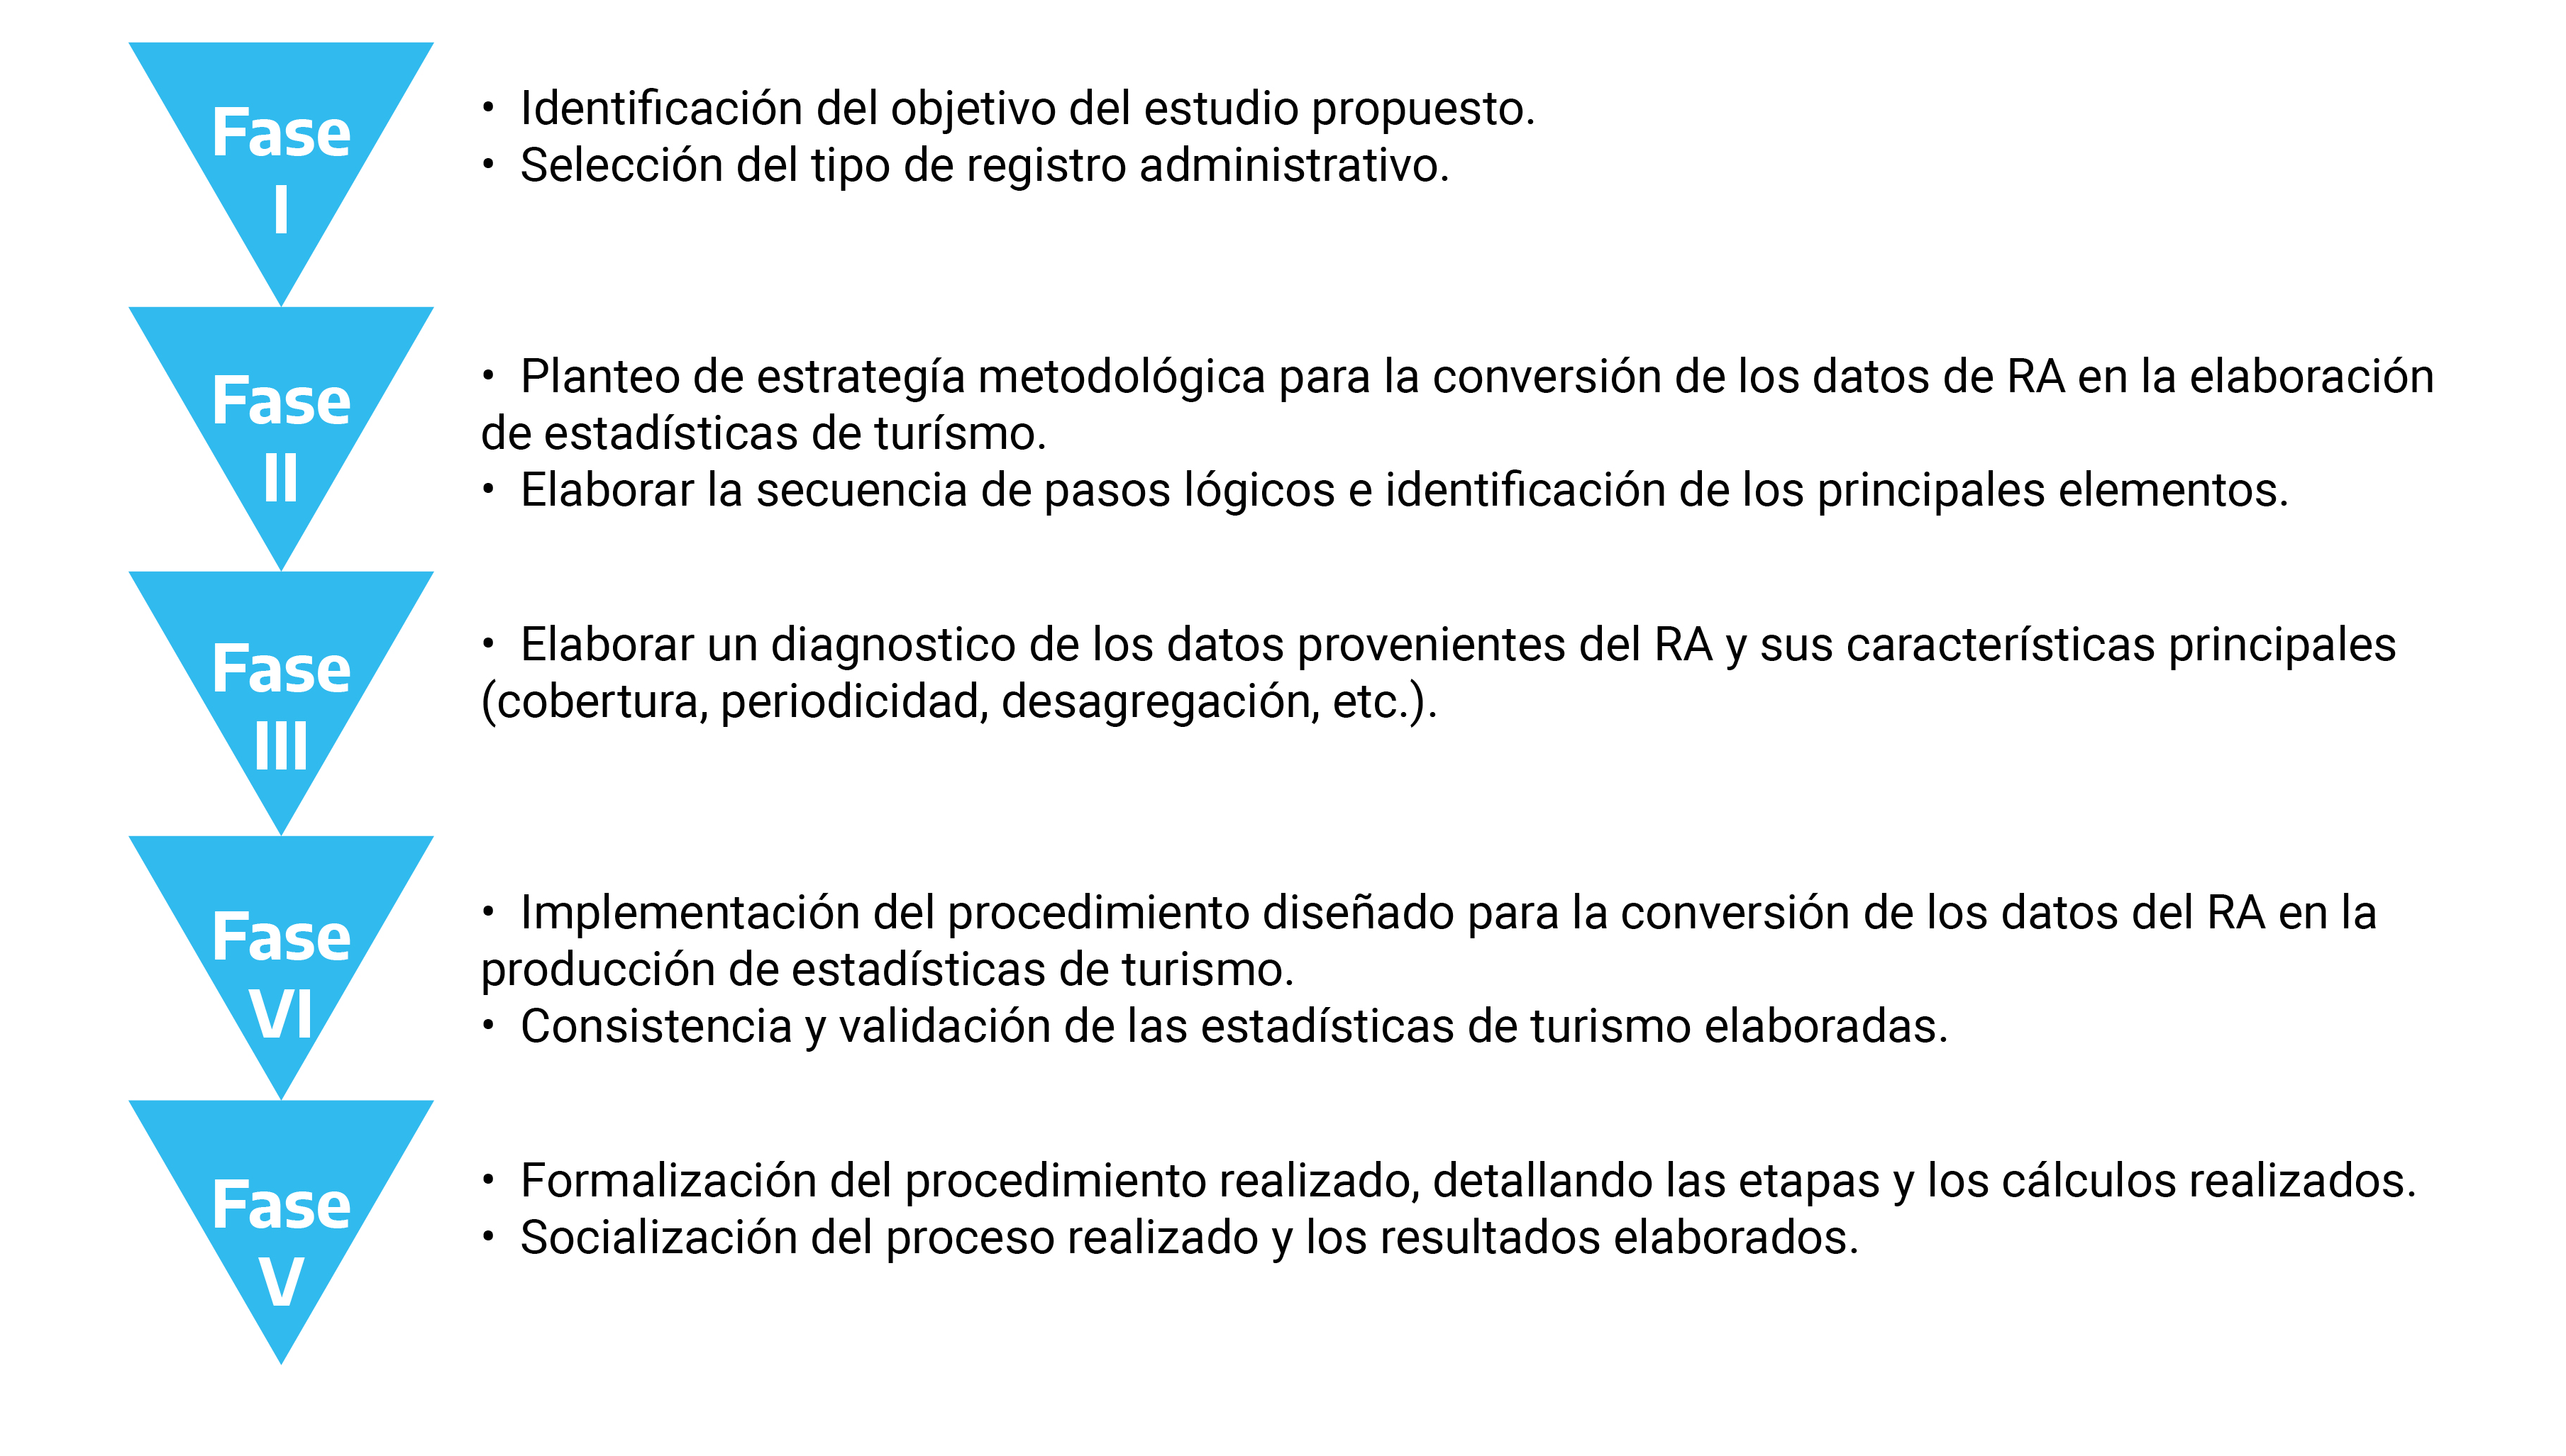
\includegraphics[width=1\linewidth]{imagenes/figura02} 

}

\caption{Fases de la conversión de datos provenientes de registros administrativos en información estadística}\label{fig:Fases}
\end{figure}

En primer lugar, en la fase I se requiere definir la población\footnote{Es el conjunto de individuos de referencia sobre el que se realizan las observaciones para luego obtener conclusiones (hacer inferencias).} objetivo y se debe contar con la máxima claridad sobre el objetivo general del estudio propuesto, ya que éste permitirá orientar los pasos subsiguientes en la correcta explotación del \texttt{RA}.

En la fase II, se plantea que la definición de dicha población requiere contemplar los siguientes elementos:

\begin{enumerate}
\def\labelenumi{\Roman{enumi})}
\item
  \textbf{Unidad Administrativa}: está compuesta por los elementos registrados en cada uno de los \texttt{RA}.
\item
  \textbf{Alcance}: se refiere a la ubicación espacial y geográfica del estudio (provincial, departamental y/o municipal).
\item
  \textbf{Tiempo}: define el intervalo de tiempo en el cual se realiza la investigación (mensual, semanal, quincenal, etc.).
\item
  \textbf{Marco Muestral}\footnote{Un marco muestral se define como una lista que contiene el conjunto de unidades (población) del cual se seleccionará la muestra a partir de la cual se realizará la inferencia estadística.}: cada uno de los \texttt{RA} podría utilizarse como marco muestral para una posterior expansión en caso de realización de alguna encuesta.
\end{enumerate}

En tercer lugar, en la fase III se deberá elaborar un diagnóstico respecto a qué tipo de datos e información suministra y almacena cada uno de los múltiples \texttt{RA}, como así, las características principales.

La fase IV, consiste en la implementación del proceso de conversión, mediante el cual se explotará la información de los registros para la producción de estadísticas de turismo y las tareas de consistencia y validación de las ET elaboradas.

Por último, la fase V resulta crucial debido a que se refiere, por un lado, a la formalización del procedimiento realizado, detallando las diferentes etapas y los cálculos exactos, y por otro lado, a la socialización y discusión de las estadísticas de turismo elaboradas.

En conclusión, no sólo resulta importante la selección del \texttt{RA} a utilizar para el análisis estadístico del sector, sino que también se deben considerar las diferentes etapas previamente planteadas para obtener información estadística robusta y atinada.

\hypertarget{situaciuxf3n-internacional}{%
\section{Situación Internacional}\label{situaciuxf3n-internacional}}

La Organización Mundial del Turismo (OMT) recomienda la utilización de los RA como una de las fuentes secundarias principales, junto a las encuestas, para la producción de estadísticas tendientes a la medición del Turismo.

En este sentido, en línea con lo comentado anteriormente, se resalta el hecho de que las estadísticas basadas en \texttt{RA} suelen ser subproductos de los procesos administrativos. Asimismo, enuncian que con frecuencia se basan en operaciones continuas, por lo que pueden ser una fuente útil de estadísticas constantes y longitudinales. Sin embargo, se reconoce el hecho de que los \texttt{RA} también pueden tener algunos inconvenientes, como una cobertura y contenido limitados, conceptos y definiciones inflexibles, falta de exhaustividad, incoherencias y un acceso limitado debido a restricciones legales o administrativas \citep{omt2010}.

A pesar de reconocer la importancia que los \texttt{RA} poseen para la confección de información estadística, no suelen hallarse recomendaciones en cuanto al procedimiento metodológico a aplicar en la búsqueda de la conversión de la información administrativa en información estadística. Por tanto, cada país se encuentra a cargo de la confección del procedimiento metodológico a aplicar a fin de realizar una óptima conversión de la información y aquí radica la importancia del presente documento.

En materia de experiencias internacionales, a modo de un sintético estado de situación, se hace referencia a experiencias denominadas como ¨buenas prácticas¨ en los usos y utilización de los \texttt{RA}.

Un caso que resulta relevante mencionar es el de España, debido a la utilización exhaustiva de los \texttt{RA} como insumo para la producción de estadísticas de Turismo. Los estudios en los que se centran, muchos de ellos realizados en la actualidad por el Instituto Nacional de Estadística (INE), son los siguientes:

\begin{itemize}
\item
  El análisis de los \texttt{RA} empleados en la Encuesta de Movimientos Turísticos en Fronteras (Frontur).
\item
  El análisis de la información de vuelos y pasajeros internacionales de Aeropuertos Españoles y Navegación Aérea (AENA).
\item
  El análisis del registro de entradas y salidas en el Museo del Prado.
\item
  El análisis de los registros de la Seguridad Social sobre el empleo en las actividades turísticas.
\end{itemize}

Por último, en Finlandia, como en varios otros países de Europa, la utilización de los \texttt{RA} se ha expandido en forma sistemática, hasta tal punto que en muchas situaciones reemplaza a los censos tradicionales. Es decir, debido a la calidad de sus \texttt{RA} en estadísticas vitales y migraciones ya no precisan la realización de censos de población para determinados estudios estadísticos. Si bien no constituye un ejemplo ligado al turismo, este caso da cuenta de cuán importante son (y, más aún, pueden ser) los \texttt{RA} bien aprovechados.

\hypertarget{situaciuxf3n-nacional}{%
\section{Situación Nacional}\label{situaciuxf3n-nacional}}

En el marco de la experiencia nacional, resulta relevante destacar la utilización de los RA sistematizados en las bases de datos de la Dirección Nacional de Migraciones (DNM) de ingresos y egresos de personas por los pasos fronterizos del país, lo cual constituye una de las fuentes principales para la estimación del turismo internacional de la Argentina. El procesamiento de dichos RA implican una serie de instancias para poder realizar la estimación de visitantes (turistas y excursionistas):
1. Eliminación de registros duplicados.
2. Identificación de viajeros tripulantes, con el fin de excluirlos de la estimación de visitantes.
3. Identificación de viajeros frecuentes, con el fin de excluirlos de la estimación de visitantes.
4. Contabilización de visitantes, identificando turistas y excursionistas en función del pernocte.
5. Estimación de la condición de residencia de los turistas y excursionistas (desde julio 2020).
Con este proceso, y junto con información obtenida de la Encuesta de Turismo Internacional (ETI), se realiza todos los meses la estimación de turismo receptivo y emisivo de la Argentina. Cabe destacar también, que dichos registros constituyen el univeso poblacional al cual se expanden los datos muestrales de la ETI.

Para mayor información consulte el informe metodológico de la estimacion del turismo internacional de Argentina:

Documento metodológico. \href{https://www.yvera.tur.ar/estadistica/informe/documentos/descarga/5dc0460bcfa3e053142696.pdf}{Estimación del turismo internacional de Argentina}

Y para mayor detalle de los conceptos básicos en la definición de visitante: \href{https://dnme-minturdep.github.io/DT1_medicion_turismo/flujo-turistico.html\#medici\%C3\%B3n}{Documento Técnico \#1}

Asimismo, desde el Ministerio de Turismo y Deportes de la Nación (MINTURDEP), se recopilan cifras sobre la cantidad de visitantes a los Parque Nacionales, dependientes de la Administración Nacional de Parques, ubicados en las distintas jurisdicciones provinciales. En su mayoría estos datos se encuentran clasificados por nacionalidad de origen (argentinos/extranjeros). Dentro de la última variable, en varios casos, los argentinos se encuentran diferenciados según tengan origen o no en la provincia en donde se encuentra el Parque Nacional en cuestión. Con esta información, el MINTURDEP elabora estimaciones estadísticas sobre visitantes a un subconjunto de los distintos parques nacionales, constituidos por una selección de 35 parques que cuentan con métodos sistemáticos de registro de visitas de las 49 áreas protegidas nacionales existentes. Es decir, no se cuenta con información sobre la totalidad de los parques nacionales existentes. No obstante, gracias a las cifras recopiladas por APN, el MINTURDEP cuenta con la posibilidad de confeccionar estadísticas importantes en relación a los flujos de visitas, de manera sistemática y confiable, dado que los datos recibidos poseen robustez gracias a la metodología mediante la cual se recaban históricamente.

Para mayor información sobre los PN podés consultar los informes mensuales publicados en:

\href{https://www.yvera.tur.ar/estadistica/informe/info/parques-nacionales}{Yvera - Parques Nacionales}

\href{http://datos.yvera.gob.ar/dataset/parques-nacionales}{Series estadísticas}

Otro RA utilizado sistemáticamente por el MINTURDEP es la base de movimientos aéreos, de cabotaje e internacional, que elabora la Administración Nacional de Aviación Civil (ANAC), y que incluye todo tipo de movimientos aéreos- regulares, no regulares, como así también aquellos movimientos correspondientes a vuelos privados, a vuelos oficiales y a maniobras. La información de esta fuente, ya sea en forma pura o en combinación con los datos de otra fuente secundaria (la base de la DNM), resulta de suma utilidad para complementar el análisis de turismo interno e internacional. La cobertura de la información de esta fuente es total, ya que capta todos los movimientos (hasta las maniobras de las escuelas de aviación). Sin embargo, acorde al objetivo de caracterizar el turismo interno e internacional, el MINTURDEP realiza un recorte de esta base, seleccionando únicamente los movimientos de un conjunto de empresas comerciales, que realizan habitualmente vuelos regulares y no regulares, ya que es probable que estos últimos transporten mayoriatariamente visitantes (aunque el ser ``pasajero'' no es sinónimo de ser ``visitante'').

Para consultar las estadísticas aerocomerciales de la Argentina podés visitar la sección de datos de la página web de la \href{https://datos.anac.gob.ar/estadisticas/}{ANAC}

Finalmente, el SIPA -Sistema Integrado Previsional Argentino- es otro RA trabajado por el \href{http://www.trabajo.gob.ar/estadisticas/}{Ministerio de Trabajo} y utilizado por el MINTURDEP para el seguimiento del empleo en el sector turístico. El SIPA contabiliza los puestos de trabajo privados asalariados registrados a nivel mensual y trimestral con distintos niveles de desagregación geográfica (nacional y provincial) y de ramas de acividad. Su utilización para la estadística de turismo es tratada en el Documento Tecnico N°5.

Por otro lado, a nivel provincial, departamental y/o municipal se utilizan múltiples \texttt{RA} tanto desde la perspectiva de la oferta como de demanda. Aun así, existe subexplotación de la información existente y, en segundo lugar, falencias con el relevamiento y procesamiento de la información.

A continuación, se listan los puntos más comunes en torno a las falencias mencionadas a fin de realizar una óptima utilización de los \texttt{RA}:

\begin{itemize}
\item
  Sub-explotación: en varios casos, no se ha reconocido la existencia de la posibilidad de extracción de mayor cantidad de datos de las fuentes secundarias. A su vez, en muchas situaciones se elaboran sistemáticamente \texttt{RA} sin fines de ser utilizados posteriormente como insumos para la producción de estadísticas.
\item
  Escaso procesamiento estadístico: como ya se ha mencionado, los \texttt{RA} no se encuentran diseñados específicamente para su explotación estadística, es decir, no suelen estar sometidos a validaciones o correcciones no estadísticas de errores. En efecto, se requiere de un procesamiento de conversión adecuado de los datos recibidos para luego poder utilizarlos en un estudio de tipo estadístico.
\item
  Falta de actualización de datos: es usual que a partir de \texttt{RA} se realicen estudios muestrales a fin de calcular coeficientes, para posteriormente llevar a cabo análisis sobre el universo bajo estudio. Éstos requieren ser actualizados, cada determinado período de tiempo, a fin de reflejar en forma más fehaciente la realidad del sector. Por ejemplo, si en el año 2019 se estiman coeficientes sobre la cantidad de individuos por automóvil que entran a una cierta localidad, éste debe ser recalculado cada una determinada cantidad de años, de acuerdo a los cambios que caben esperarse. Esto se debe a que la situación del sector turístico no es uniforme a lo largo de los años. Con el paso del tiempo podrían registrarse variaciones, positivas y/o negativas respecto del flujo turístico hacia las distintas localidades, aun cuando se mantenga constante el flujo vehicular, pero la cantidad de personas promedio podría disminuir.
\item
  Falta de incorporación de la estacionalidad del sector en los estudios estadísticos: los coeficientes también deben ser ajustados según el momento turístico del año en cada jurisdicción. En todas las provincias, departamentos y/o municipios, se pueden reconocer sub-periodos de mayor o menor afluencia turística (temporada alta/baja), dentro de un mismo año, y cada uno merece un tratamiento especializado. Al reconocer la estacionalidad y la elasticidad frente a las condiciones socioeconómicas que posee el sector turístico, se resalta la importancia que la actualización de las estimaciones poseen. Así, resulta importante contar con un calendario turístico, de modo de identificar los momentos que pertenecen a períodos de mayor o menor movimiento de visitantes.
\end{itemize}

En síntesis, se debe evaluar la posibilidad de realización de estudios sencillos y acotados ejecutados de la forma más eficiente y con el menor despliegue de recursos, que permitan luego, a partir de los datos que brinda el \texttt{RA}, realizar una estimación de las cantidades y de ciertas características de los visitantes.

En el capítulo siguiente, se presenta y propone una clasificación de los \texttt{RA}, con el propósito de orientar la identificación de cada uno de ellos según: el tipo de información que proporciona y su fuente de información, la perspectiva de oferta y demanda, según su alcance y, por último, su utilización.\\
~\\

\hypertarget{clasificaciones}{%
\chapter{\texorpdfstring{\textbf{Clasificaciones}}{Clasificaciones}}\label{clasificaciones}}

Uno de los múltiples objetivos del proyecto de Armonización de las Estadísticas de Turismo en las Provincias consiste en la elaboración de un estado de situación actualizado de la recopilación y sistematización de los \texttt{RA} existentes a nivel provincial, departamental y/o municipal.

A partir de la información relevada en las jurisdicciones provinciales, se reflexiona sobre los distintos tipos de \texttt{RA} utilizados en cada una de ellas, las cuales poseen distintos grados de cobertura y confiabilidad. Los mismos se obtienen tanto de entes públicos como privados.

En primer lugar, en las provincias existe una gran cantidad de entes generadores de datos a partir de los registros de entradas y salidas por distintos medios de transporte: terrestre, acuático y/o aéreo. En general, de la información de las entradas y salidas de vehículos, dichos entes procuran estimar la cantidad de visitantes, en base a coeficientes o estimaciones indirectas.

La robustez de estos registros presenta un alto grado de disparidad entre sí, ya que mientras en algunos casos cuentan con un registro de tipo censal, como son los aeropuertos; otros son de tipo muestral, como por ejemplo, algunos controles policiales en ruta que registran las entradas y salidas de automóviles en determinados momentos. La disparidad se incrementa cuando se trata de visitantes, debido a que se ha dado cuenta de que si bien existen registros de tipo censal, al igual que el caso anterior, otros son realizados en base a ponderaciones aplicadas a las muestras de servicios de transporte mencionadas anteriormente.

Asimismo, se verifica que los organismos que calculan las estadísticas de turismo en aquellas provincias que cuentan con Parques Nacionales y/o Provinciales, reciben, con distinta periodicidad, los registros de ingresos de visitantes a los mismos. En este caso, las cifras obtenidas poseen un cierto grado de sistematicidad y confiabilidad ya que en su mayoría las cifras se obtienen a partir de los tickets vendidos y/o conteos de ingresantes. Una situación análoga ocurre con los ingresos registrados por los atractivos turísticos culturales, como ser museos y centros históricos, y los de tipo recreativos como por ejemplo: aerosillas, parques temáticos, etc.

Se da cuenta también de que algunas provincias realizan estimaciones acerca de la cantidad y utilización de las segundas viviendas existentes. Este cálculo es de gran importancia para el análisis del turismo rutinario o frecuente. Hasta el momento, sólo se ha verificado una estimación a partir de los registros provenientes de las Empresas de Servicios Públicos, más específicamente de la electricidad.

Por último, se verifica la importancia que poseen aquellas fuentes secundarias que permiten obtener cifras de empleo en el sector turístico. Las mismas pueden obtenerse tanto de fuentes públicas (agencias de recaudación) o privadas (prestadores de servicios turísticos). La importancia que se les atribuye a este tipo de registros se debe a que dichos datos ofrecen un panorama de la generación de puestos laborales en el sector, lo cual implica un gran impulso económico para la provincia en su totalidad.

La clasificación de los \texttt{RA} permite elaborar diferentes perspectivas de análisis que facilitan identificar, categorizar y/o agrupar a los múltiples registros existentes. A continuación se detallan cuatro formas de clasificación respecto del objetivo de la categorización de los \texttt{RA}.

Las perspectivas de clasificación propuesta corresponden, en primer lugar, a qué tipo de información almacena y cuáles son las fuentes de información que suministran dichos registros; en segundo lugar, desde la perspectiva de oferta y/o demanda, en relación al acceso a la información; en tercer lugar, según el alcance; por último, según la utilización que se realiza de ellos.

\hypertarget{seguxfan-tipo-de-informaciuxf3n}{%
\section{Según tipo de información}\label{seguxfan-tipo-de-informaciuxf3n}}

Se elaboró una primera tipología de clasificación que identifica el tipo de información que los diferentes \texttt{RA} almacenan y proporcionan, como así también, cuáles son las fuentes de información que suministran los respectivos \texttt{RA}. Se presentan cinco agregados desde los cuales al interior de cada uno de ellos se realizan sub-desagregaciones que procuran desarrollar analíticamente cada una de las dimensiones para la producción de estadísticas de Turismo.

En primer lugar, el Transporte, agrupa a tres tipos: Terrestre, Aéreo y/o Acuático.

\begin{figure}

{\centering 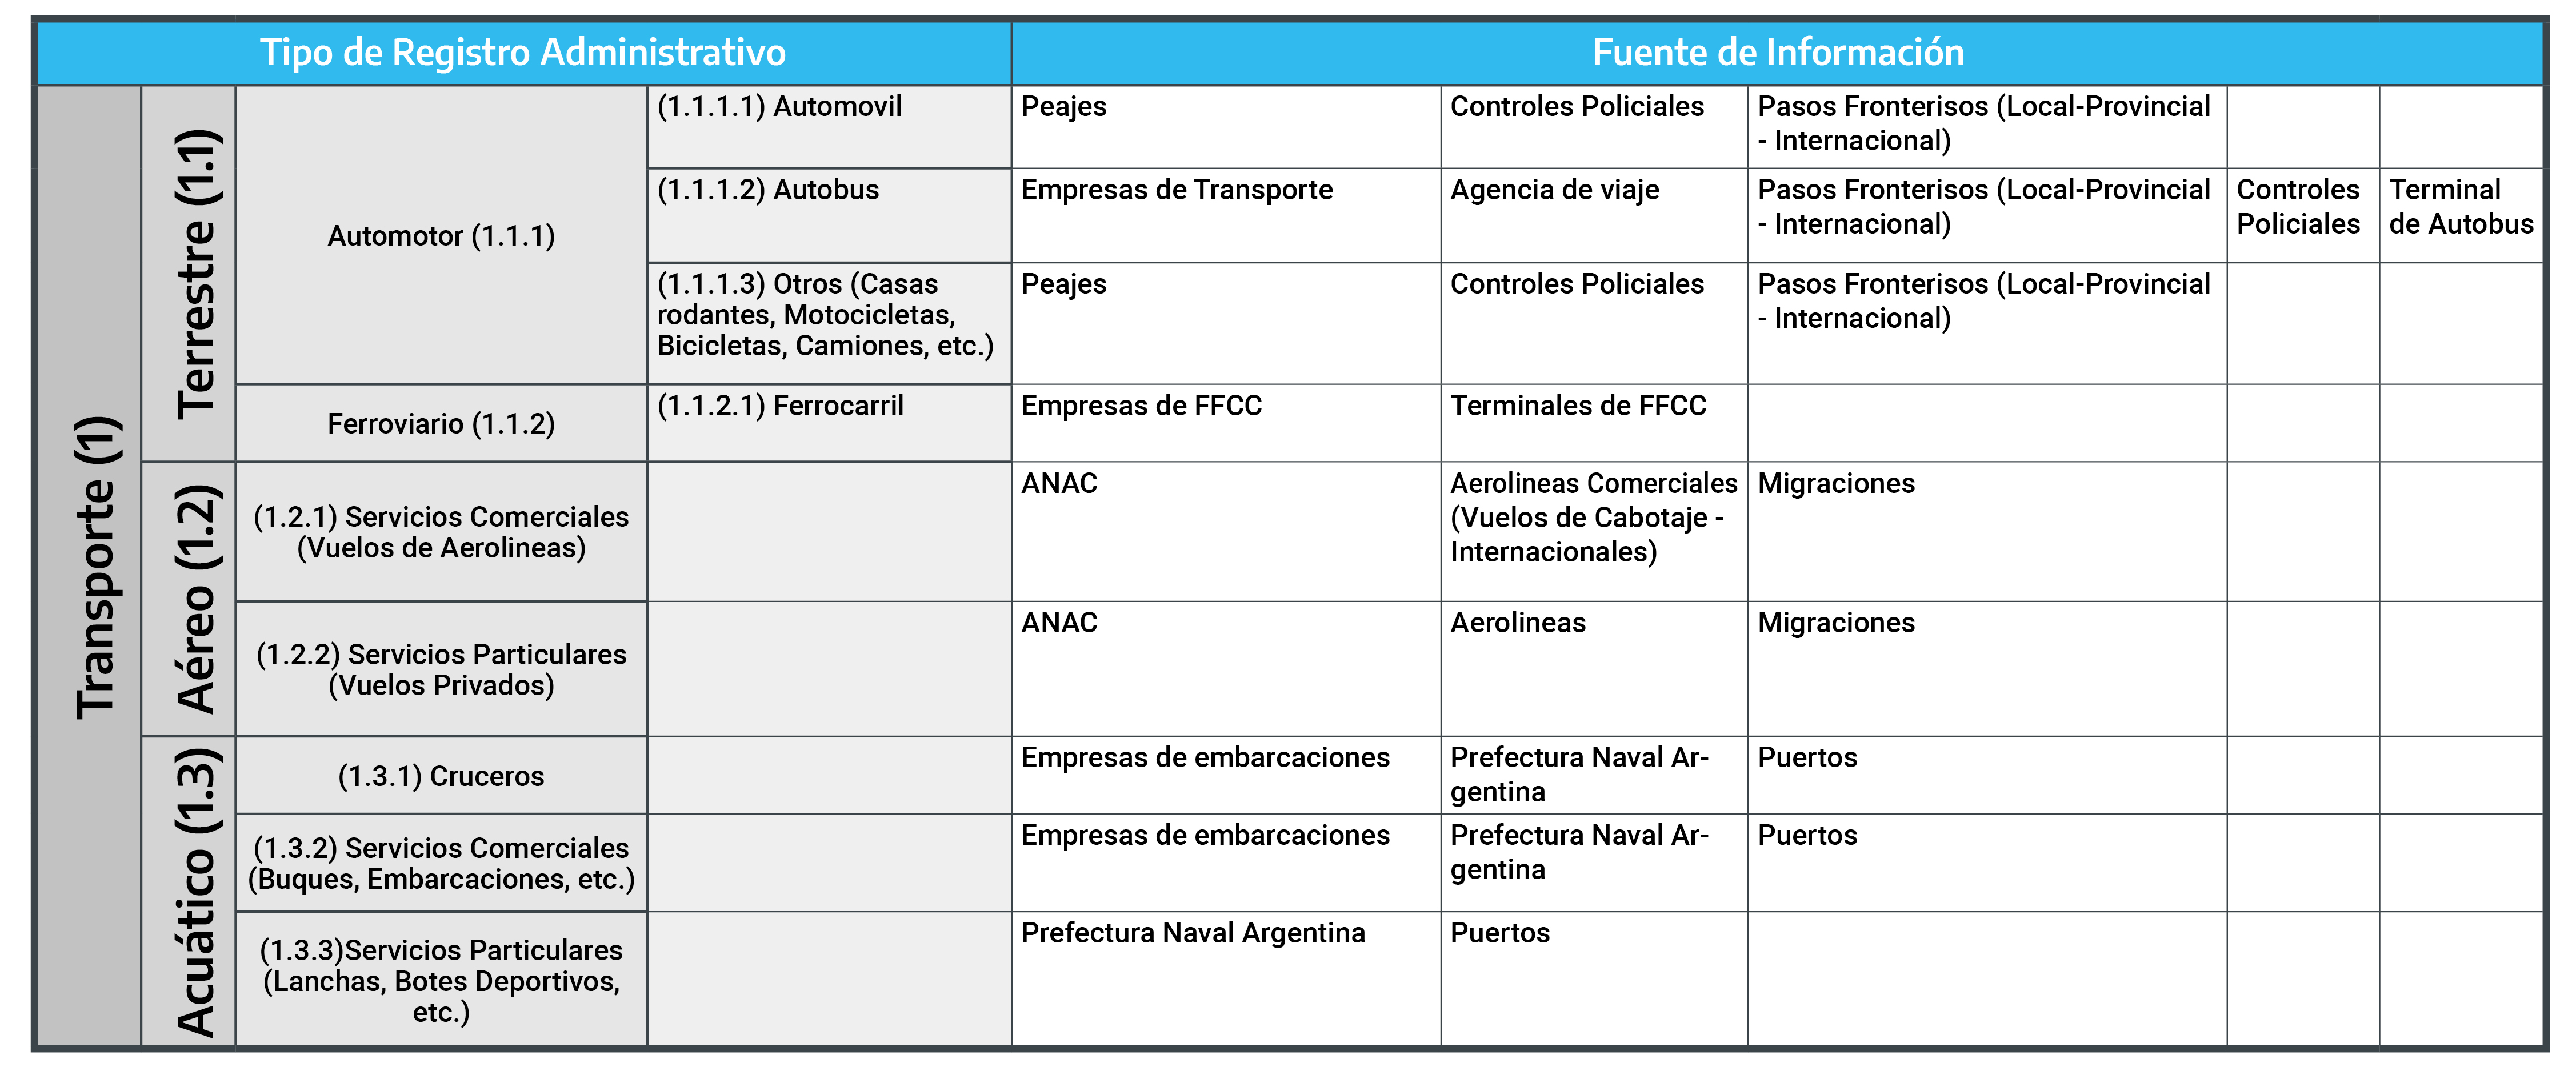
\includegraphics[width=1\linewidth]{imagenes/figura03A} 

}

\caption{Clasificación de los registros administrativos ligados al transporte por tipo de información}\label{fig:clasificaciontransporte}
\end{figure}

En segundo lugar, los Atractivos Turísticos, contemplan a los Naturales, Culturales y/o Recreativos. Luego, en tercer lugar, la Oferta Turística (Figura \ref{fig:clasificacionatractivos}), incluye a los prestadores y oferentes de productos y/o servicios turísticos.

\begin{figure}

{\centering 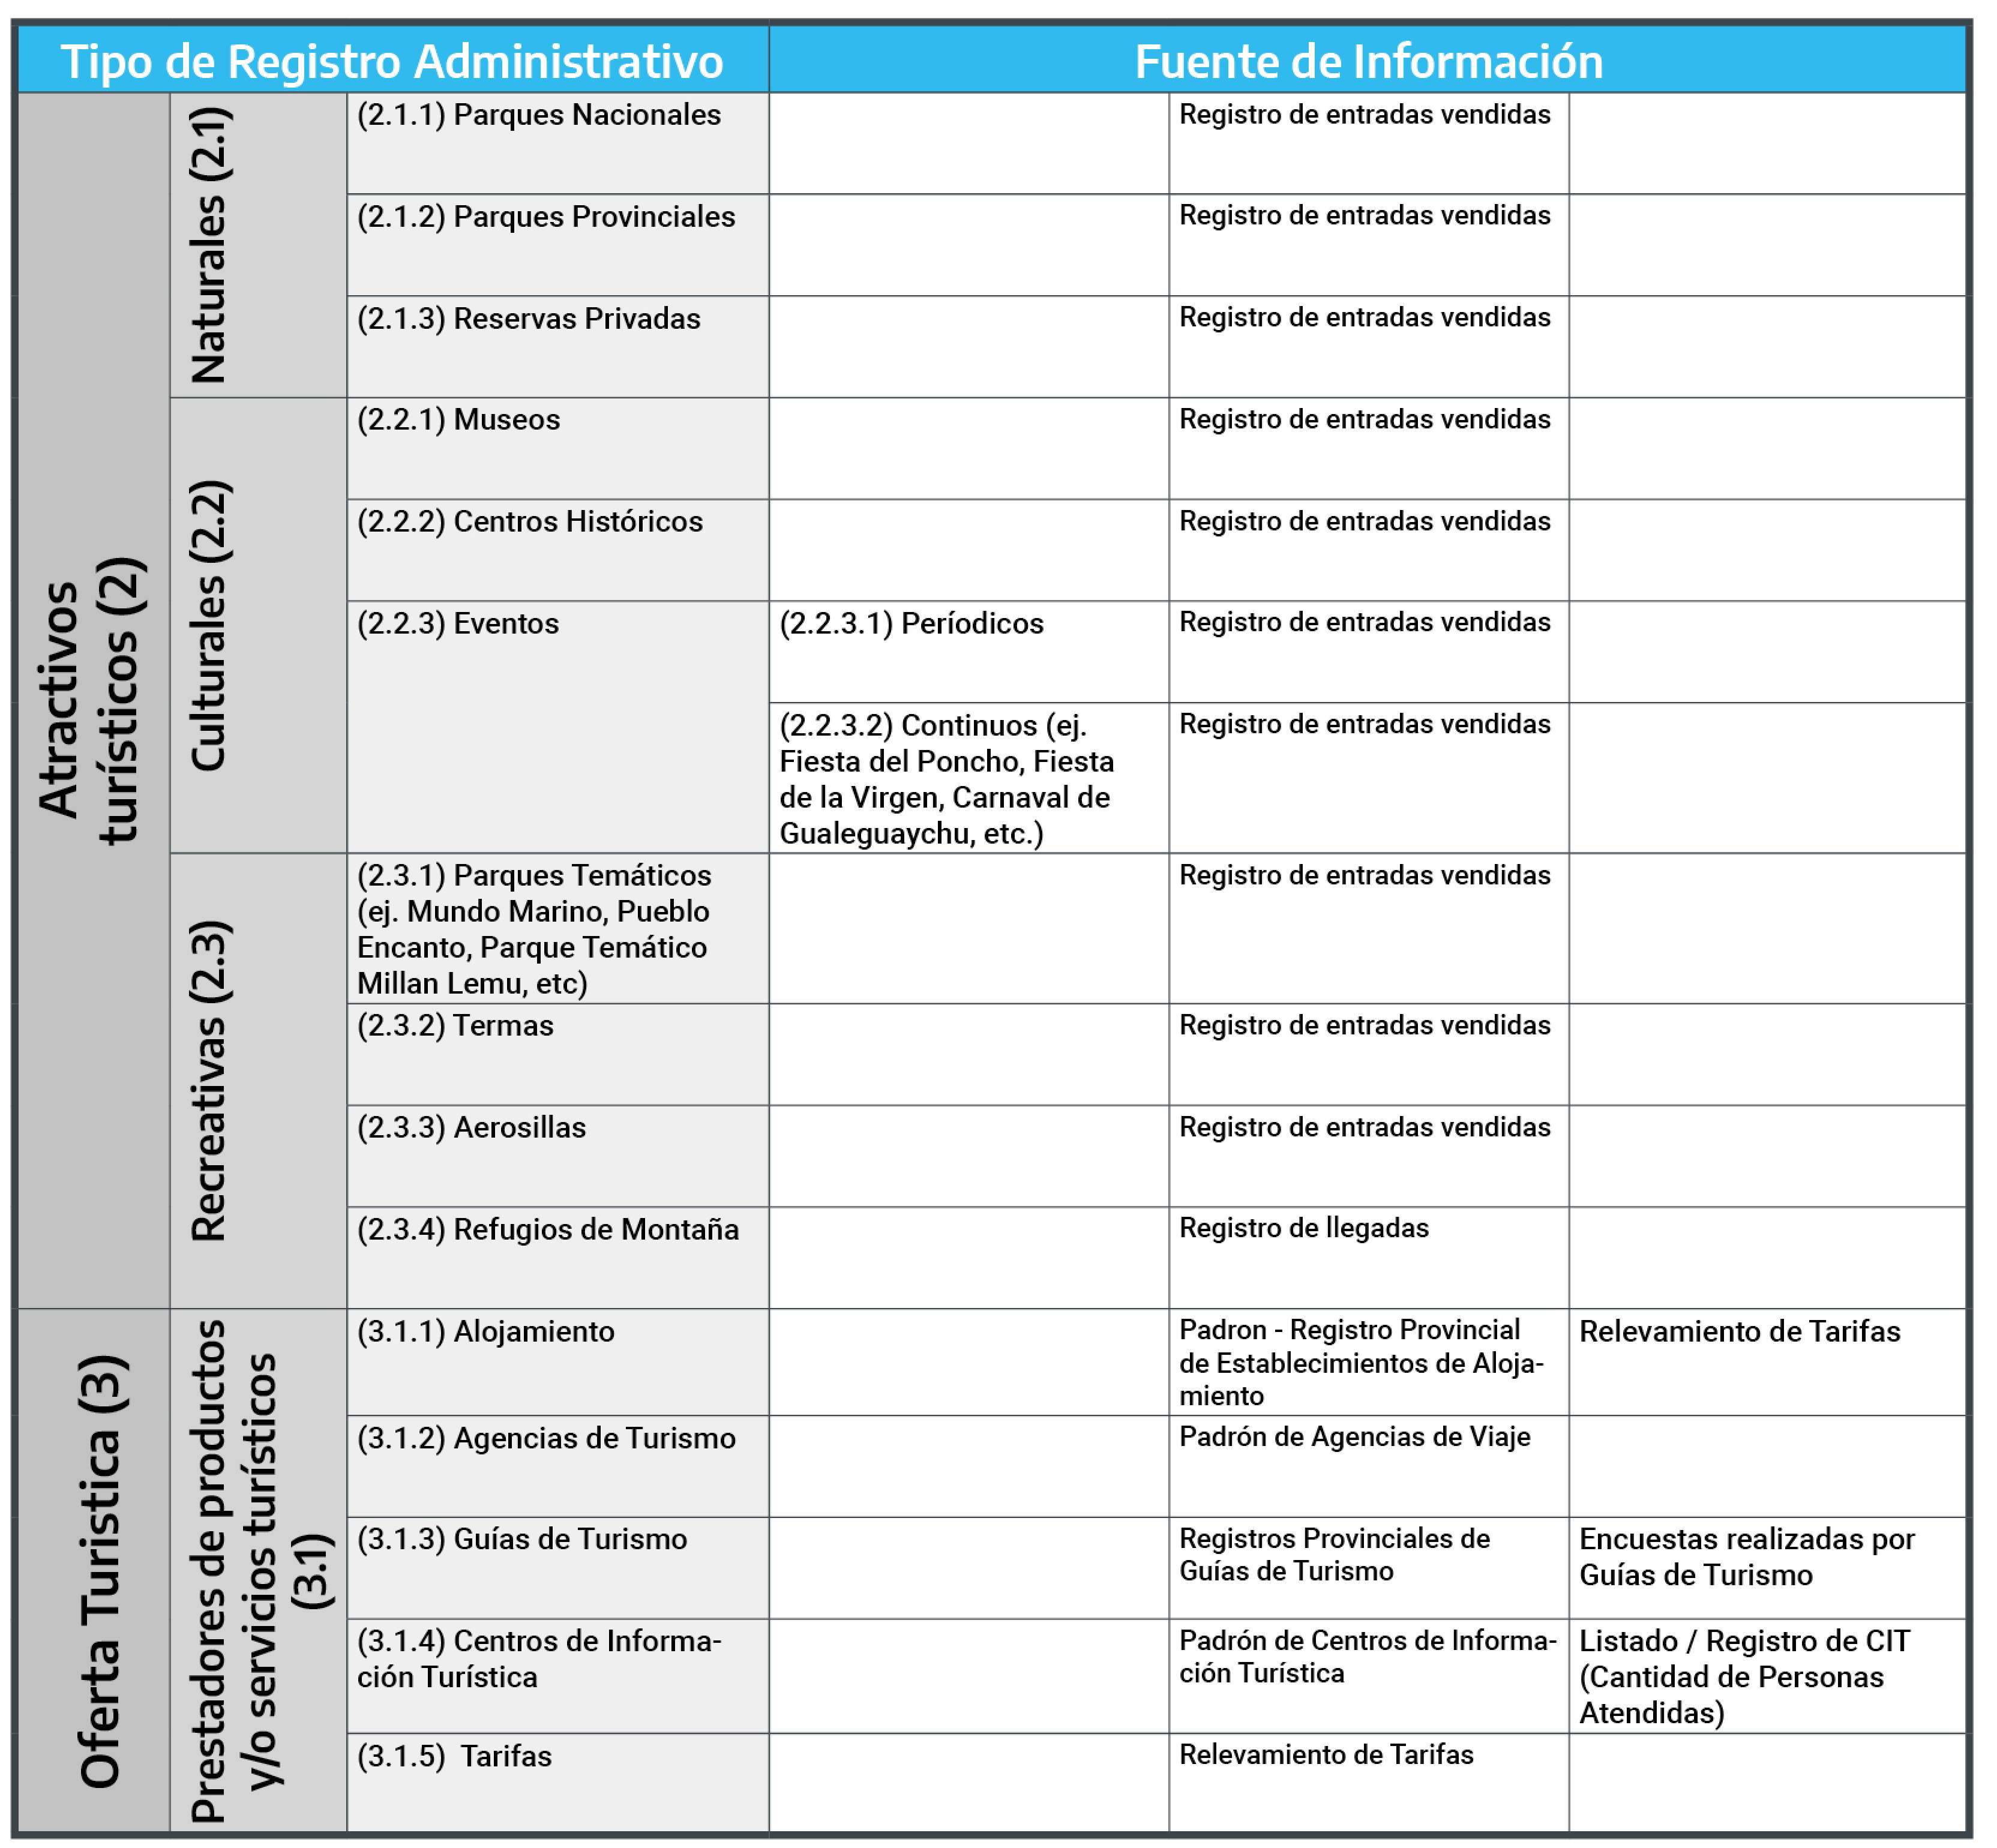
\includegraphics[width=1\linewidth]{imagenes/figura03B} 

}

\caption{Clasificación de los registros administrativos ligados a los atractivos turísticos y a la oferta turística por tipo de información}\label{fig:clasificacionatractivos}
\end{figure}

En cuarto lugar, las Segundas Viviendas, únicamente debido a su especificidad propia. Por último, en quinto lugar, la cuantificación del Empleo (Figura \ref{fig:clasificacionsegundasviviendas}), respecto del tipo de gestión que suministra la información.

\begin{figure}

{\centering 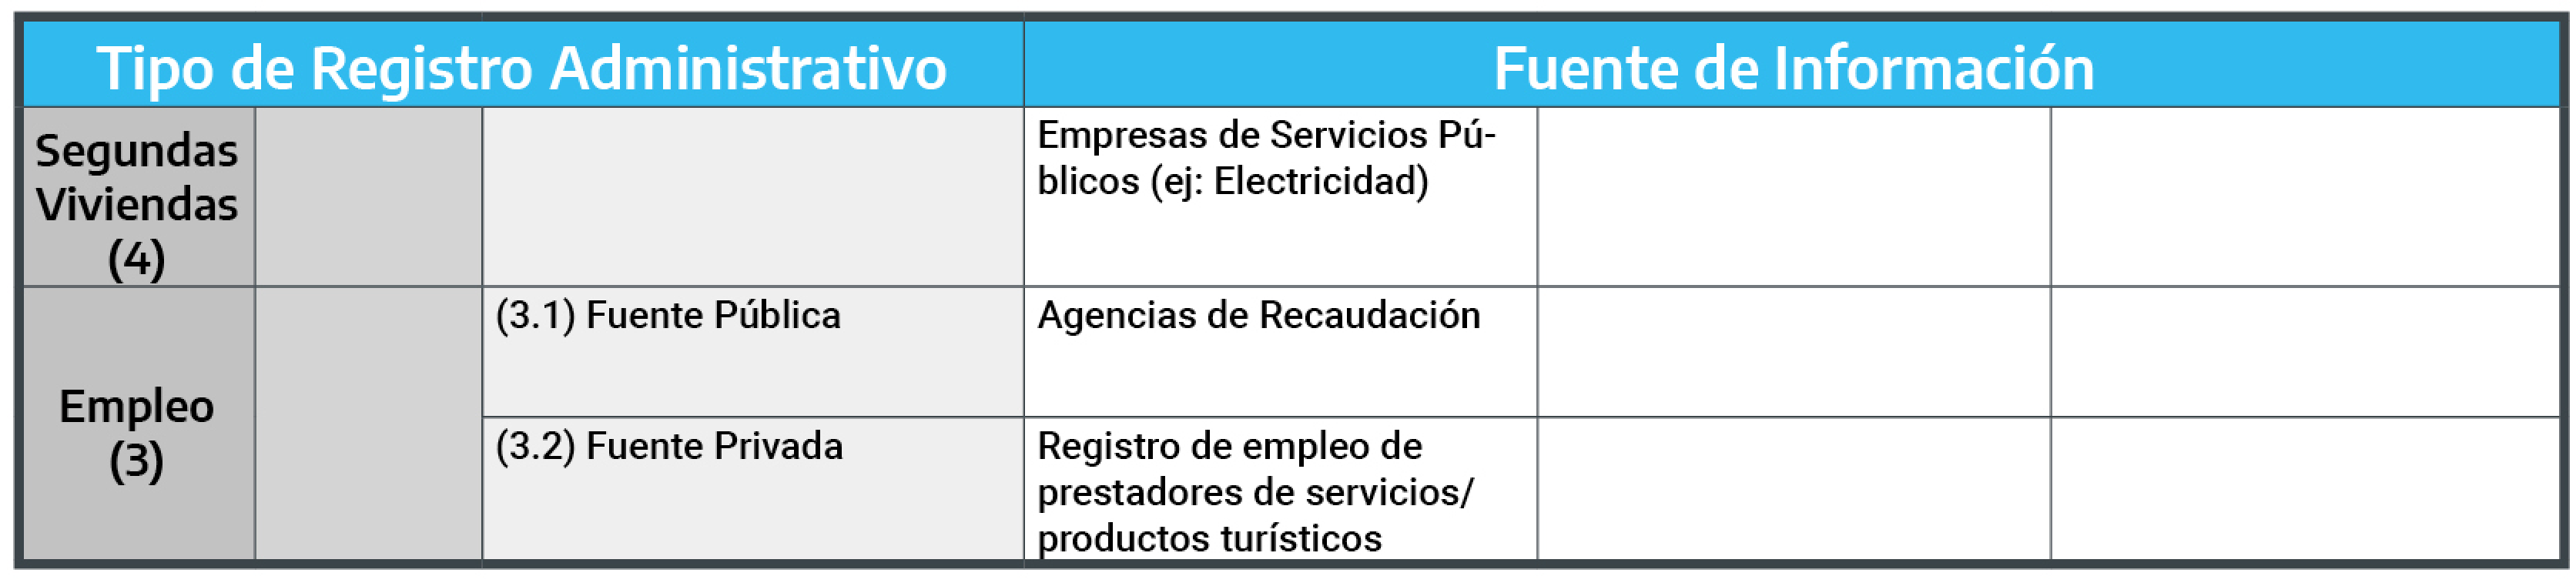
\includegraphics[width=1\linewidth]{imagenes/figura03C} 

}

\caption{Clasificación de los registros administrativos ligados a las segundas viviendas y al empleo por tipo de información}\label{fig:clasificacionsegundasviviendas}
\end{figure}

\hypertarget{seguxfan-ofertademanda}{%
\section{Según oferta/demanda}\label{seguxfan-ofertademanda}}

Una segunda forma de clasificación posible de los \texttt{RA} parte de la perspectiva o enfoque desde la porción del mercado turístico de la que se brinda información. Es decir, si está ligado a la demanda (actividades, consumos, etc. realizados por los visitantes) o a la oferta (unidades productoras o prestadoras de bienes y servicios).

En efecto, desde la demanda, las unidades informantes (públicas y/o privadas) más comunes son:

\begin{itemize}
\item
  Empresas de Peaje
\item
  Terminales (Ómnibus, Aéreas y/o FF.CC) -- informando sobre cantidad de visitante que ingresan y/o egresan de las unidades geográficas
\item
  Centros de Información Turística (CITs)
\end{itemize}

Atractivos:

\textbf{I)} Naturales (Parques Nacionales, Provinciales)

\textbf{II)} Culturales (Museos, Centros Históricos, Eventos)

\textbf{III)} Recreativos (Parques Temáticos, Termas, Aerosillas, etc.)

En cambio, desde la perspectiva de la oferta, se podría agrupar a las unidades informantes tales como:

\begin{itemize}
\item
  Terminales (Ómnibus, Aéreas y/o FF.CC) -- informando sobre cantidad de servicios que ingresan y/o egresan a la unidad geográfica;
\item
  Registro y/o Padrón de Establecimientos de Alojamiento Turístico (dependiente de la Provincia, Departamentos y/o Municipios);
\item
  Agencias de Turismo;
\item
  Guías de Turismo.
\end{itemize}

Cabe señalar que esta distinción entre oferta y demanda no siempre resulta clara y/o tajante. Así, si se construye un padrón de hoteles con cantidad de habitaciones y tipo de servicios, se está accediendo a información que caracteriza a la oferta, pero si, además, se cuenta por ejemplo con información sobre facturación, ello resultará indicativo de la demanda. Una situación análoga puede encontrarse en el caso del transporte público (asientos o lugares disponibles y ocupados).

Por último, se encontró otras fuentes claves de información como ser la cantidad de Segundas Viviendas proveniente del Censo Nacional de Población, Hogares y Viviendas y la generación de Empleo siendo información suministrada por unidades públicas y/o privadas.

\hypertarget{seguxfan-alcance}{%
\section{Según alcance}\label{seguxfan-alcance}}

En tercer lugar, resulta relevante considerar el ``alcance'' de los múltiples \texttt{RA}, respecto de contemplar claramente e identificar qué tipo de información sistematizan y almacenan cada uno de los mismos.

En efecto, se podría clasificar como parcial y/o total la información proporcionada por cada uno de los registros. El alcance, deberá considerarse para la expansión de los resultados elaborados y, en base a ellos se proyectará a la población total que se procure medir y cuantificar.

Por ejemplo, se pueden encontrar \texttt{RA} de tipo parcial como ser las personas que visitaron algún atractivo turístico de una determinada provincia, ya que esta información permite visualizar sólo a una porción del universo total de visitantes, (quienes ingresan a los atractivos) que podrían arribar a dicha provincia. Por lo tanto, la información de dicho registro claramente representa sólo una porción y, por ende, si el objetivo es conocer el total de visitantes, se deberá contemplar algún proceso de conversión de forma tal que permita expandir dicho valor al total.

En cambio, entre aquellos de tipo total se pueden encontrar a los provenientes de accesos a la provincia, municipio y/o departamento, los cuales posibilitan una aproximación, con relativa significatividad, respecto de la medición del total de la afluencia turística. Por ejemplo, en una determinada provincia, los peajes y/o puestos camineros, al registrar el total de servicios (tanto privados --automóviles, camiones, motocicletas, casas rodantes, etc.-, como públicos --ómnibus-) según frecuencia y capacidad total de traslado de personas cuentan con vasta información de ingresos y egresos de las personas a dicha jurisdicción. No obstante, la limitación que presenta dicho registro, es la imposibilidad de diferenciar a los visitantes (turistas y/o excursionistas) del total de personas trasladadas, para lo cual, se requerirá realizar un operativo estadístico que permita cuantificar dicha magnitud.\\

\hypertarget{seguxfan-utilizaciuxf3n}{%
\section{Según utilización}\label{seguxfan-utilizaciuxf3n}}

En cuarto lugar, interesa resaltar la importancia de contemplar la utilización de la información de los registros de manera Directa o Indirecta en el marco de la medición del Turismo.

La utilización de los \texttt{RA} se refiere a la posibilidad (o imposibilidad) de sus usos tal cual se encuentra almacenada la información de los mismos. En decir, si el mismo se utiliza tal cual fue elaborando, si se lo emplea como un insumo para un proceso de producción estadística posterior o si se lo usa para la elaboración de coeficientes de distribución, etc.

Como ya se ha señalado, la utilización de los registros en general requiere un proceso de conversión estadística, que transforme a las unidades administrativas en unidades estadísticas, lo cual sugiere una utilización indirecta de los mismos (por ejemplo, la cantidad de vehículos es un insumo para estimar la cantidad de visitantes).

Asimismo, existe la posibilidad de la utilización directa. Por ejemplo, en un Centro de Información Turística (CIT) de un departamento y/o municipio, el recuento de las personas que ingresan solicitando información, podría expresarse como la cantidad de visitantes al CIT en un momento determinado. No obstante, dicha cantidad no representa en forma directa la cantidad de visitantes a la localidad y, por lo tanto, no es metodológicamente válido, generalizar sin más dicha cantidad al total de visitantes respectivamente.

En este sentido, para la utilización de los \texttt{RA} se debe contemplar varias cuestiones previas a su explotación como fuente de información secundaria. Qué tipo de información proporciona, cómo se almacena y acumula la misma, qué tipo de procesamiento estadístico debe realizar para poder utilizarse como indicadores de medición del Turismo, entre otras.

En síntesis, las clasificaciones presentadas se proponen como una primera propuesta de ordenamiento de los diferentes \texttt{RA}, en base a la información registrada por cada uno de ellos, en el marco de las experiencias recopiladas mediante las visitas técnicas a las jurisdicciones provinciales del país.

Resulta importante destacar que, existe una subexplotación de los \texttt{RA} como fuente secundaria de información para la producción de ET. En el capítulo cuarto se presenta en detalle de manera analítica en base a la primera forma de clasificación planteada ``Clasificación por tipo de Registro Administrativo'' .

Dicha situación se vincula directamente a la escasa articulación institucional de las áreas de producción de ET con las diferentes unidades proveedoras de dichos registros.

También, existe un reducido desarrollo de innovaciones respecto de la utilización, con criterios metodológicos, de la información de los diferentes registros con una fuerte impronta de su utilización de forma directa como indicador de medición del Turismo, cuyas limitaciones se han desarrollado previamente.

Lo que se procura proponer mediante el desarrollo de la clasificación, y en base a sus diferentes perspectivas, consiste en la toma de conciencia sobre la existencia y disponibilidad de los múltiples \texttt{RA} y el incentivo para su solicitud y posterior tratamiento estadístico con el fin de mejorar y complejizar los operativos de estadísticas en marcha, desarrollados y/o a comenzar en las diferentes jurisdicciones provinciales.

\hypertarget{algunos-ejemplos}{%
\chapter{\texorpdfstring{\textbf{Algunos ejemplos}}{Algunos ejemplos}}\label{algunos-ejemplos}}

De los datos provenientes de registros administrativos en estadística de turismo

A partir de las experiencias provinciales se presentan algunos ejemplos de abordaje metodológico para la elaboración y producción de estadística a partir datos que pueden obtenerse desde distintos \texttt{RA} .

En primer lugar, tal como se mencionó anteriormente, siempre que se trabaje con algún \texttt{RA} debe tenerse en cuenta cuál es la población objetivo a la cual éste hace referencia. Esto resulta importante, esencialmente, para los registros de entradas a atractivos turísticos (naturales, culturales y/o recreativos). Por ejemplo, si una provincia cuenta con cifras sobre tickets vendidos en un Parque Nacional, la oficina generadora de estadísticas del turismo debe tener presente que se está haciendo referencia sólo a los visitantes a dicho atractivo y no resultaría posible su expansión al total provincial de manera directa.

A su vez, si se cuenta con un registro sobre entradas y salidas por un acceso terrestre X, pero además en la provincia existen otros accesos de los cuales no se posee registro alguno, se deberá tener presente que en este caso tampoco se hace referencia a la totalidad de los visitantes en la provincia, sino a los ``visitantes en la provincia que ingresan por el acceso terrestre X'' .

En general, se observa una escasa explotación de los múltiples registros existentes como fuente de información accesible en los diferentes niveles institucionales. Ello implica la necesidad de un proceso de concientización respecto a la utilidad y la disponibilidad de los mismos para la elaboración de estadísticas.

En los apartados subsiguientes, se proponen algunos esquemas de tratamiento de los \texttt{RA} , procurando identificar las particularidades, ventajas, limitaciones y la información que cada uno ofrece y que hacen que, en consecuencia, se deban diseñar e implementar alternativas metodológicas específicas de conversión de los datos registrados en información turística.

Resulta frecuente encontrar que las áreas destinadas a la producción de ET utilizan distintos \texttt{RA} favoreciendo cuantificar la evolución, el comportamiento y las perspectivas del sector Turismo. Sin embargo, se ha registrado cierta subexplotación de estos. A su vez, se puede advertir sobre posibles faltas de procedimientos metodológicos sólidos para el procesamiento de datos provenientes de los \texttt{RA} . Por ello, a continuación se presentan, a través de ejemplos, alternativas de tratamientos para la conversión de las unidades administrativas en datos estadísticos.

\hypertarget{empresas-de-peajes}{%
\section{Empresas de Peajes}\label{empresas-de-peajes}}

Una de las principales fuentes secundarias de información en base a \texttt{RA} consiste en las empresas de peajes que se encuentran localizadas en diferentes puntos carreteros y vías de ingreso a las provincias, departamentos y/o municipios que resultan de gran utilidad como insumo para la elaboración de estadísticas de turismo. Cabe señalar que puestos de control vehicular (policiales, sanitarios) con registros continuos y rigurosos cumplen una función análoga a la de las estaciones de cobro de peaje.

Los datos suministrados por las firmas de peajes presentan limitaciones en su utilización directa como indicador estadístico de turismo, debido a que sólo contabilizan la cantidad de vehículos que pasan por un determinado punto. Por lo tanto, se requiere de una estrategia metodológica (proceso de conversión) específica para su utilización como insumo en la construcción de indicadores de turismo.

Acorde a la secuencia previamente presentada (en la Figura N° 2) suponiendo que la ubicación geográfica de un puesto de peaje es la vía de acceso a tres localidades distintas, A, B y C, y una de ellas requiere conocer cuál es la cantidad de arribos de visitantes, para lo cual solicita (y accede) a los \texttt{RA} del puesto de peaje.

La localidad ¨C¨ cuenta con mayor capacidad institucional para implementar un operativo in situ con el propósito de generar la información necesaria para elaborar coeficientes de distribución, que le permitan cuantificar efectivamente la cantidad de arribos de vehículos que ingresan a su localidad y, a la vez, relevar algunas variables que le permitan estimar la cantidad de visitantes, turistas y/o excursionistas.

Un elemento importante radica en que dicha localidad deberá generar una distribución específica, dentro del total de vehículos que pasaron por el puesto, para cuantificar la cantidad de vehículos que se dirigen a la misma y, posteriormente, cuantificar la cantidad de visitantes, sean turistas o excursionistas, que posean dicho destino.

Entonces, en primer lugar, se implementó una encuesta durante tres periodos: i) temporada alta (diciembre a marzo), ii) fines de semana largos y iii) fuera de temporada (abril a noviembre, excepto fines de semana largos), con el objetivo de lograr ajustar la estacionalidad, variable siempre fundamental en la medición del Turismo.

El muestreo fue aleatorio y sistemático (uno de cada X autos que pasaban por el puesto de peaje en el momento del relevamiento), con un tamaño de 600 casos para cada uno de los tres periodos. El universo contemplado fueron los automóviles y camionetas particulares (es decir, por ejemplo no se contemplaron los ómnibus). Las preguntas realizadas indagaron por la cantidad de personas por auto, el lugar de residencia habitual, el destino del viaje\footnote{A los fines de no complejizar el ejercicio, se asume que todos los vehículos que cruzan el puesto de peaje se dirigen a una de las tres localidades contempladas} y la duración de la estadía en la localidad de destino.

Los resultados de este estudio permitieron determinar, para cada uno de los tres periodos, el porcentaje de autos que arriba a cada localidad, el promedio de pasajeros por auto a cada localidad, para el total de pasajeros por localidad, la proporción de residentes y de visitantes, diferenciados en turistas (cuando pernoctan en el destino) y en excursionistas (cuando no pernoctan). Aplicando estos resultados a la totalidad de automóviles que cruzan en cada periodo el puesto de peaje (\texttt{RA} suministrado por la empresa), es posible estimar el total de visitantes (distinguiendo turistas y excursionistas) que arriban a cada una de las tres localidades por esta vía a lo largo de un año.

Por otro lado, se cuenta con información proporcionada por la empresa de peajes. Ésta informó que durante el año ingresó la siguiente cantidad de vehículos (automóviles y camionetas particulares) por el puesto:

\begin{itemize}
\item
  Temporada alta (diciembre a marzo): 70.000
\item
  Fines de semana largo: 18.500
\item
  Resto del año (abril a noviembre excepto fines de semana largo): 35.000
\end{itemize}

La Figura N° 3.1 muestra los resultados del estudio, cuya obtención se detalla a continuación.

\begin{figure}

{\centering 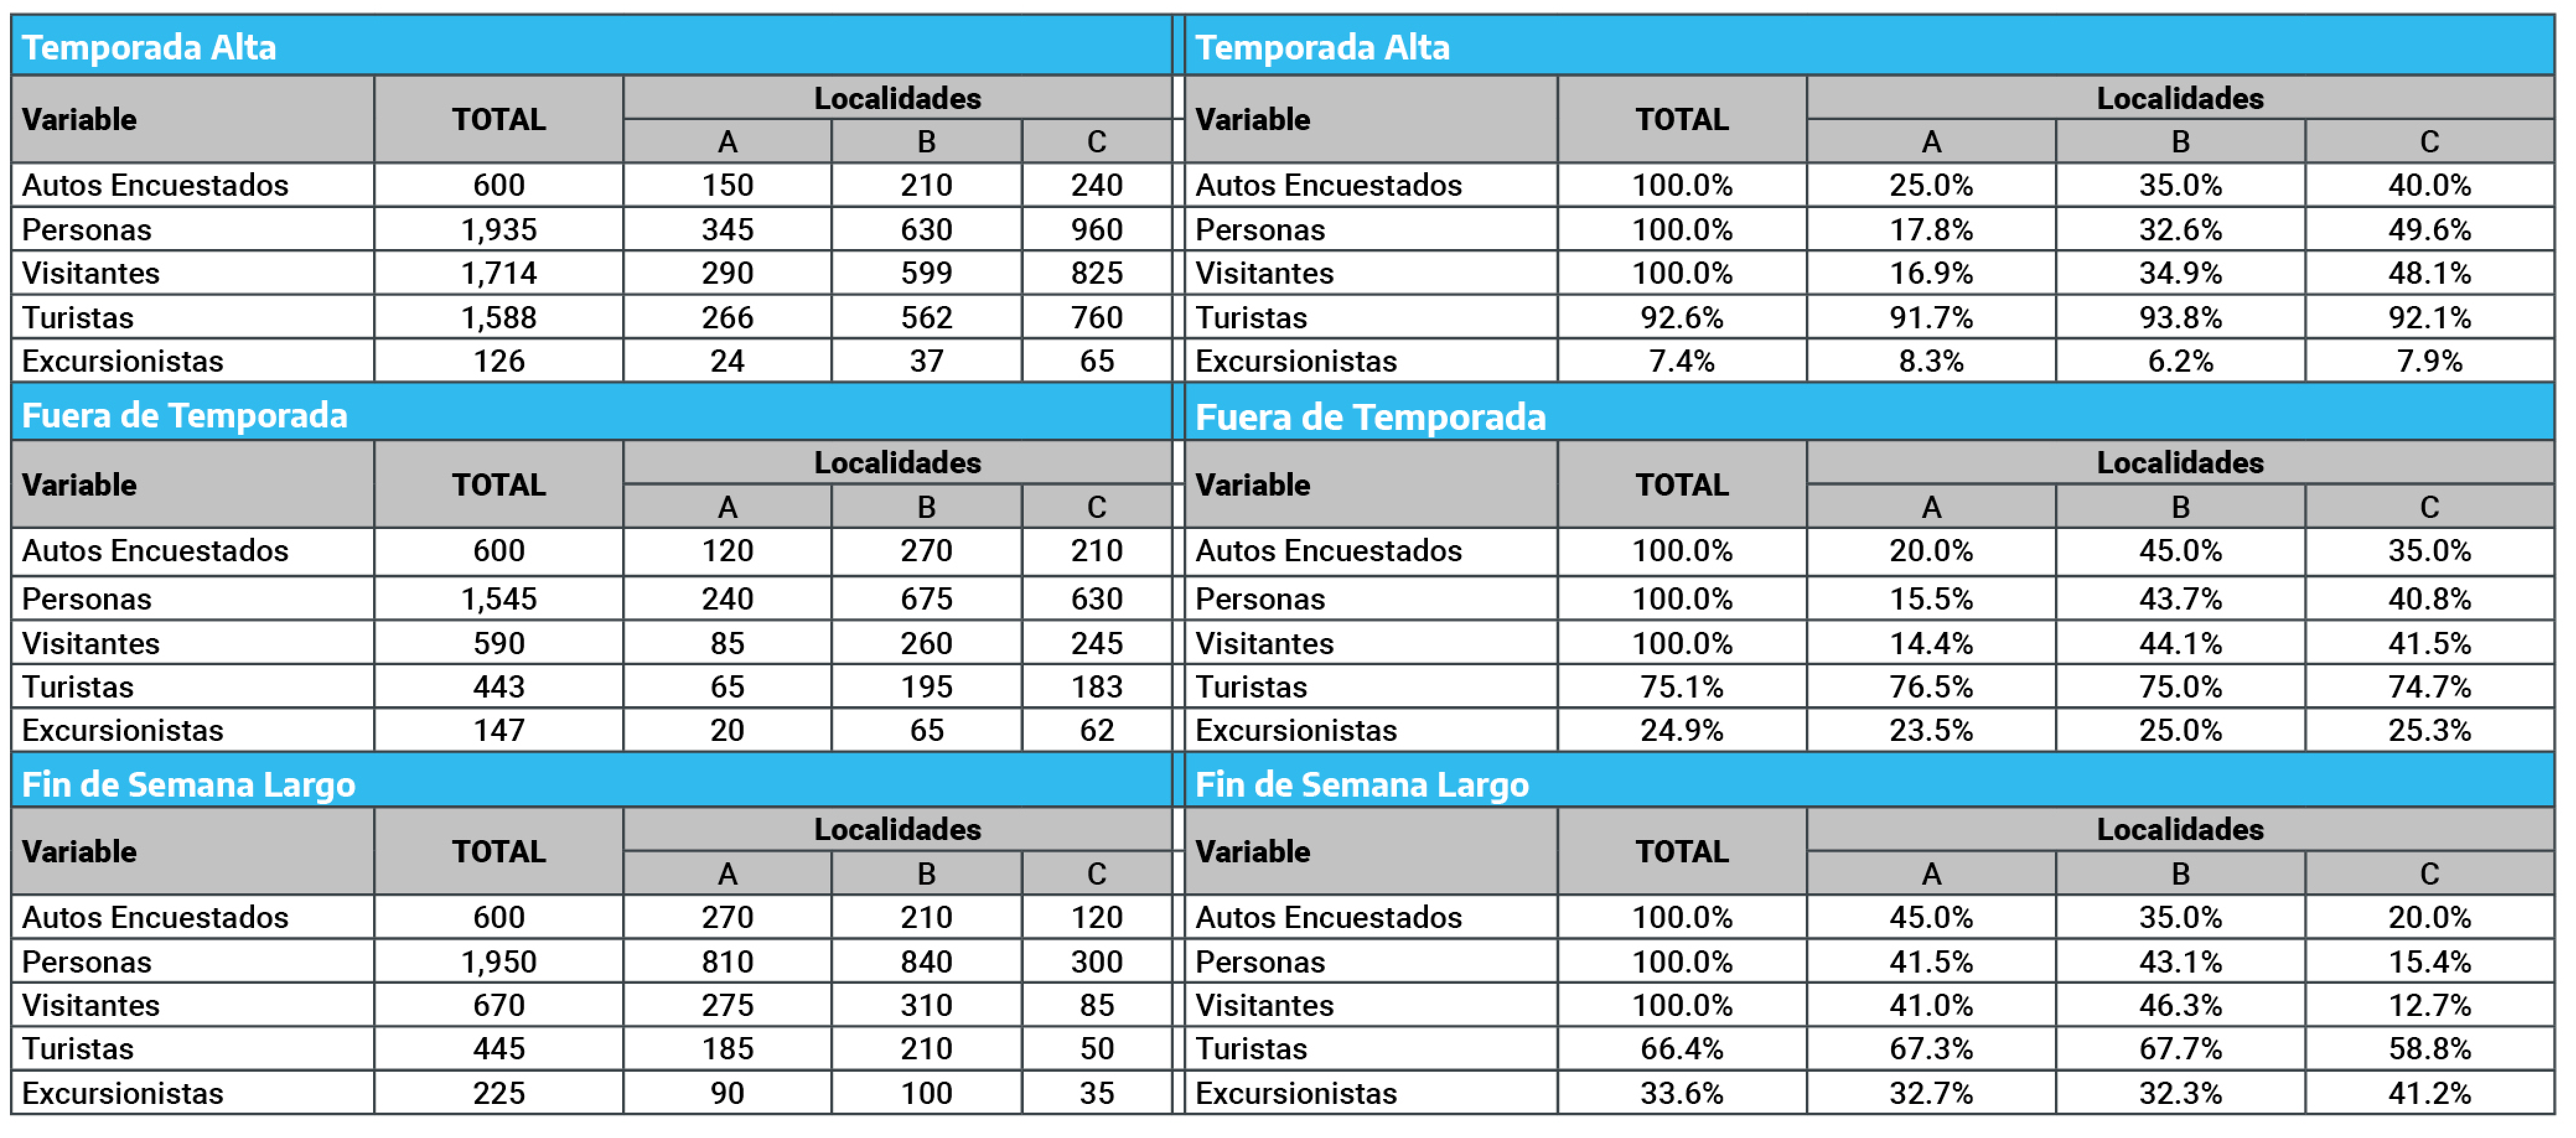
\includegraphics[width=1\linewidth]{imagenes/figura04} 

}

\caption{Resultados del estudio realizado por la localidad C}\label{fig:estudioslocalidade}
\end{figure}

El primer paso, consistió en diferenciar la localidad de destino. De la encuesta implementada, 600 casos en total, se desprendió que 150 vehículos (\(25\%\)) fueron con destino a la localidad \emph{A}, 210 (\(35\%\)) a la \emph{B} y 240 (\(40\%\)) a la localidad \emph{C}.

La cantidad promedio de pasajeros por vehículo a cada localidad, fue de 2,3 personas hacia \emph{A} (345 personas en 150 vehículos), 3,0 personas hacia \emph{B} y 4,0 personas hacia la localidad \emph{C}. Este dato resulta relevante si es que se busca aplicar dichos coeficientes a futuras estimaciones. Para este punto resulta relevante tener presente las necesidades de actualización mencionadas en el primer capítulo.

Fuera de Temporada Alta (entre abril y noviembre, sin contar los fines de semana largos) del estudio implementado, se desprende que el \(20\%\) fueron con destino a la localidad \emph{A}, el \(45\%\) a la \emph{B} y el \(35\%\) a la localidad \emph{C}, con una cantidad promedio de pasajeros de 2,0 por vehículo hacia \emph{A}, 2,5 hacia \emph{B} y 3,0 hacia \emph{C}.

Como se puede observar, la diferencia entre ambos periodos de temporada radica tanto en la proporción de vehículos que tiene como destino cada localidad (por ejemplo, a la localidad A se dirige el \(25\%\) de los vehículos de temporada alta y el \(45\%\) de los de fuera de temporada), como en la cantidad de pasajeros promedio por vehículo (siguiendo con la localidad A, 2,3 personas en temporada alta y 2,0 personas fuera de temporada).

La empresa informó un tránsito de 18.500 vehículos en todos los fines de semana largos del año, aunque el estudio se realizó en sólo uno de ellos\footnote{En este ejemplo se redujo a la existencia de un solo fin de semana largo, para evitar extender el razonamiento. Naturalmente, se deberá testear si hay o no diferencias sustanciales entre distintos fines de semana (por la época del año, por su extensión, etc.). para procurar registrar mejor la estacionalidad de los mismos.}. De la encuesta implementada, se desprende que 270 (\(45\%\)) fueron a la localidad \emph{A}, 210 (\(35\%\)) a la \emph{B} y 120 (\(20\%\)) a la \emph{C} y con una cantidad promedio de 3 personas por vehículo hacia \emph{A}, 4,0 hacia \emph{B} y 2,5 personas hacia la localidad \emph{C}.

En segundo lugar, respecto de la residencia habitual, en cada caso se consultó si era residente o no de la localidad a cuyo destino se dirigía, para poder determinar cuántas de esas personas eran visitantes. Se asumió que los visitantes cumplían con los requisitos de la definición de entorno habitual\footnote{El mismo se define como la zona geográfica (aunque no necesariamente contigua) en la que la persona realiza sus actividades cotidianas habituales (reside y trabaja). No existe una definición exacta del entorno habitual brindada por la OMT, razón por la cual se presentan diferencias entre los distintos países. Sin embargo, se debe tener en consideración que existen dos criterios claves para su definición: distancia y frecuencia. Es decir, si el individuo se desplaza a una zona geográfica de corta distancia al lugar de donde reside y/o trabaja o lo hace con una frecuencia alta, se considera que éste no ha salido de su entorno habitual. Distinto ocurre si el mismo se desplaza a una zona que se encuentra a una distancia larga o con una frecuencia baja. Por ejemplo, la Encuesta de Viajes y Turismo de los Hogares (EVyTH) define y operacionaliza el entorno habitual de un individuo que se encuentra conformado por: los lugares situados dentro de un determinado radio de la ciudad / localidad donde reside el individuo (Se consideraron 40 Km. para la región del Gran Buenos Aires -la Ciudad de Buenos Aires más los Partidos que forman parte del Conurbano Bonaerense- y 20 Km. para el resto del país), o los visitados una o más veces por semana por el mismo, aunque estén situados a una distancia mayor a la ya mencionada.} para diferenciarse de las personas con residencia local.

Por ejemplo, en la Temporada Alta, la cantidad total de visitantes que cruzaron por el peaje fue de 1.714 (sobre un total de 1.935 personas contabilizadas), de los cuales 290 tuvieron como destino la localidad \emph{A} (266 turistas y 24 excursionistas -es decir, que no pernoctaron-) 599 la localidad \emph{B} (562 turistas y 37 excursionistas), y por último, 825 a la localidad (760 turistas y 65 excursionistas).

Asimismo, el relevamiento que contempló el periodo fuera de Temporada Alta y de los fines de semana largos, contabilizó, en los 600 autos que participaron del estudio, de 590 visitantes(sobre 1.545 personas que viajaban en estos vehículos, lo que muestra la preponderancia de residentes que se cuentan en este periodo): 85 a la localidad A (65 turistas y 20 excursionistas), 260 a la localidad \emph{B} (195 y 65 respectivamente), y por último, 245 visitantes a la localidad \emph{C} (183 turistas y 62 excursionistas).

Por último, durante el fin de semana largo contemplado en el estudio, la cantidad total que surge del estudio sobre 600 vehículos arroja un total de 670 visitantes: 275 visitantes a la localidad \emph{A} (185 turistas y 90 excursionistas), 310 a la localidad \emph{B} (210 turistas y 100 excursionistas), y 85 a la localidad \emph{C} ( 50 turistas y 35 excursionistas).

Es importante observar que los diferentes coeficientes de distribución elaborados varían en los tres periodos de tiempo considerados.

Una vez elaborados los coeficientes en base al estudio, estos se deben aplicar a la cantidad total de vehículos, informados por la empresa, que cruzaron el puesto de peaje en cada uno de los tres periodos considerados. De ese modo, se obtendrá el total de visitantes (turistas y excursionistas por separado) para cada una de las localidades.

Como se podrá observar en la Figura 3.2, en la Temporada Alta el total de vehículos ingresados ha sido de 70.000 y que el \(25\%\) se dirigió a la localidad \emph{A}, \(35\%\) a la localidad \emph{B} y \(40\%\) a la localidad \emph{C}, se puede concluir que en dicho período los automóviles que las localidades recibieron fueron, 17.500 (\(70.000\)*\(25\%\)), 24.500 (\(70.000\)*\(35\%\)) y 28.000 (\(70.000\)*\(40\%\)), respectivamente.

\begin{figure}

{\centering 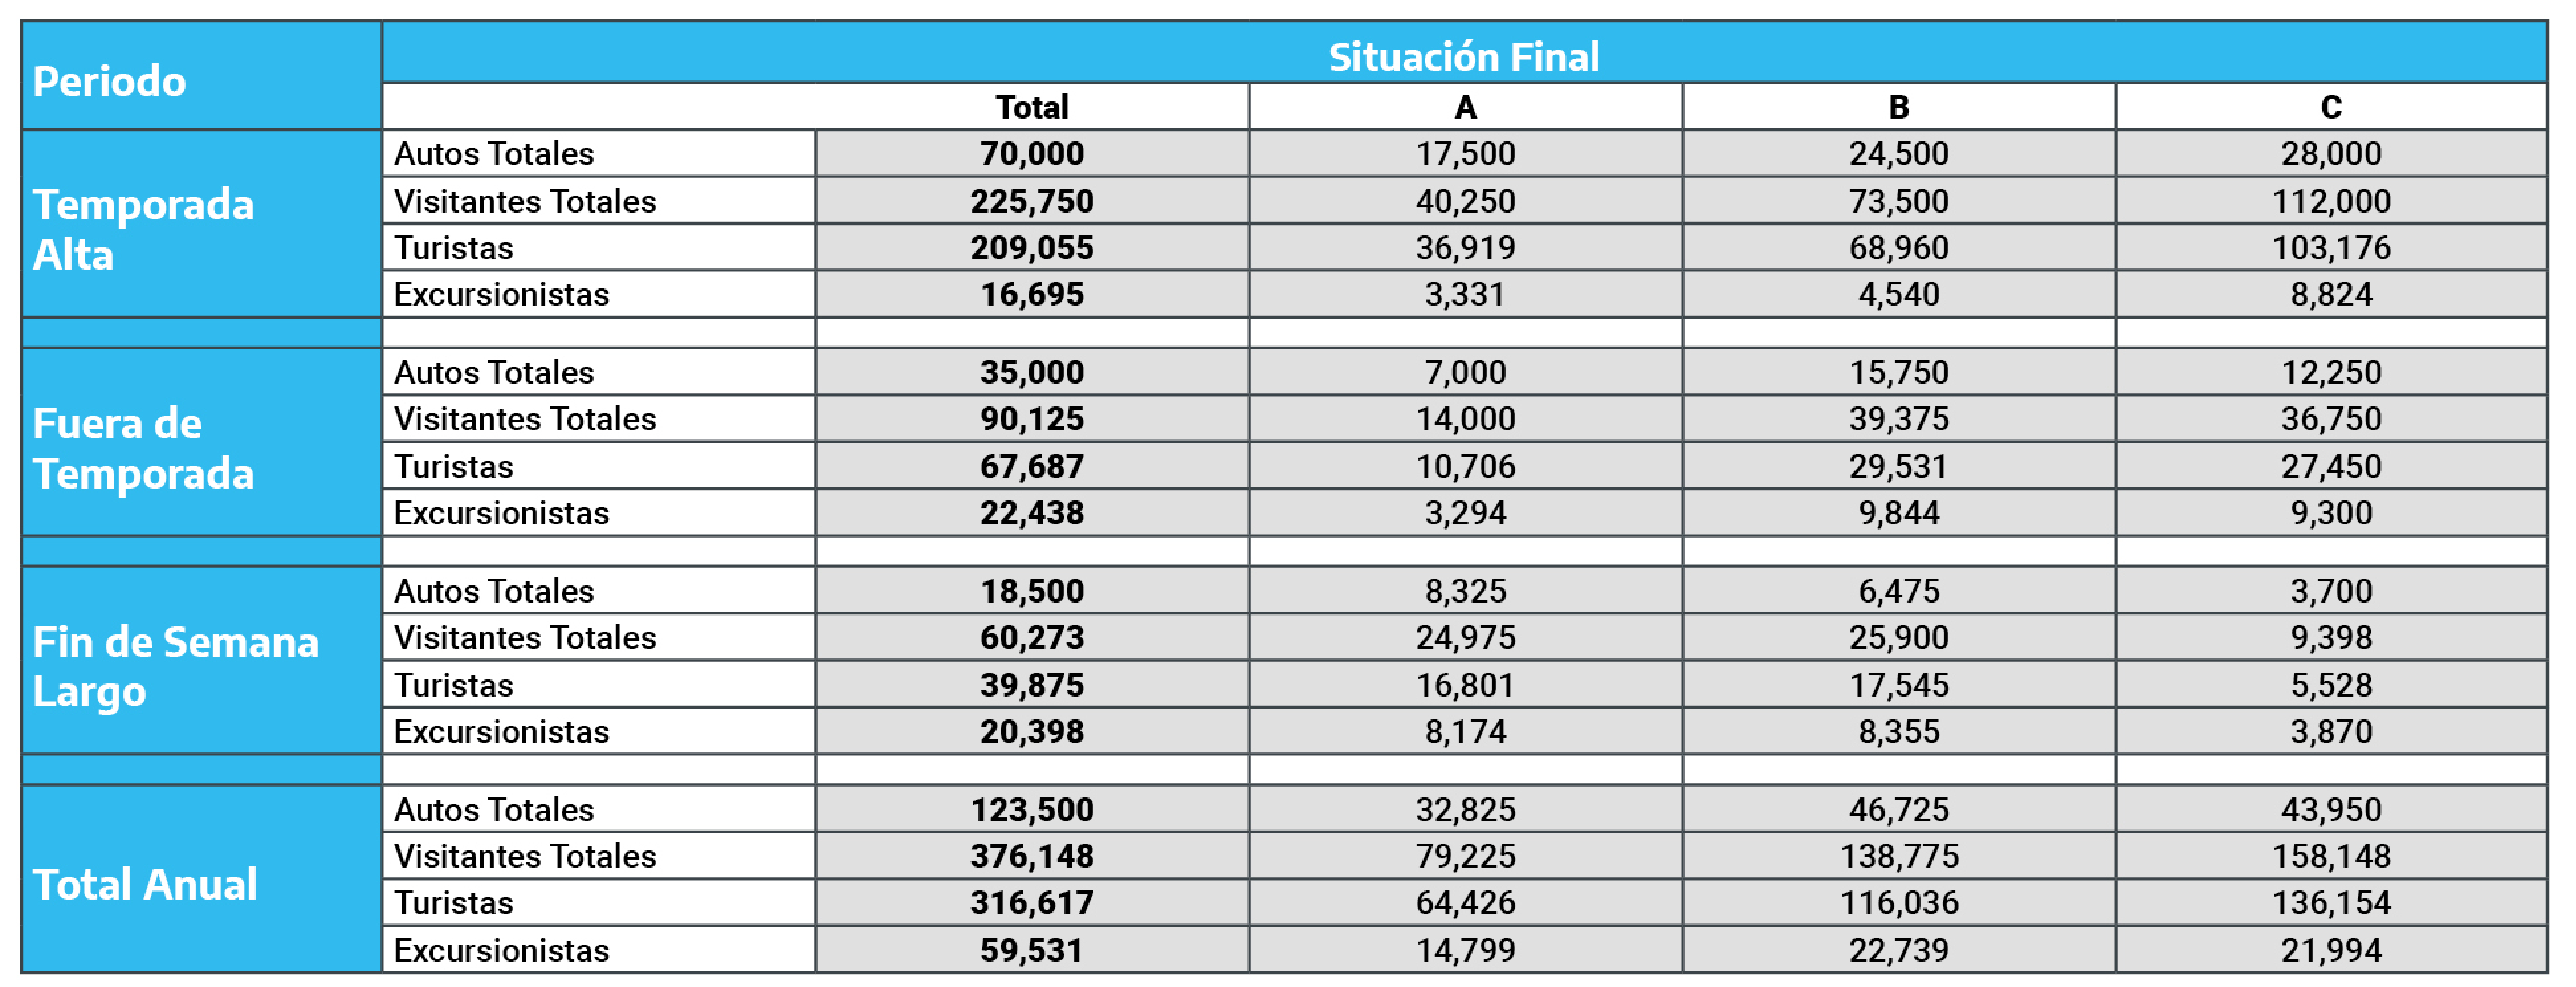
\includegraphics[width=1\linewidth]{imagenes/figura5A} 

}

\caption{Coeficientes del estudio realizado por la localidad C aplicados a los totales informados por la empresa de peaje}\label{fig:coeficientes}
\end{figure}

El hecho de realizar tres estudios (uno para cada periodo temporal) indudablemente implica una erogación mayor que realizar sólo uno. No obstante, sólo de esta manera es posible reflejar fielmente la realidad y, más aún, poder realizar estudios longitudinales (comparación de llegadas de visitantes en distintos años, por ejemplo), que suele ser un objetivo común de las estadísticas de turismo\footnote{Si bien aquí no se entra en detalle sobre las cuestiones a tener en cuenta en el diseño de las muestras requeridas para los estudios planteados, pues el objetivo es llamar la atención sobre los procesos de construcción lógica de la información, en otros documentos elaborados en el marco del proyecto de Armonización de las Estadísticas de Turismo en las Provincias se desarrolla exhaustivamente, desde distintos ángulos, esta temática.}.

La Figura 3.3 permite comparar los resultados obtenidos más arriba con los que hubiesen surgido si se hubiese aplicado a las cantidades de vehículos de cada periodo los coeficientes correspondientes a la temporada alta.

\begin{figure}

{\centering 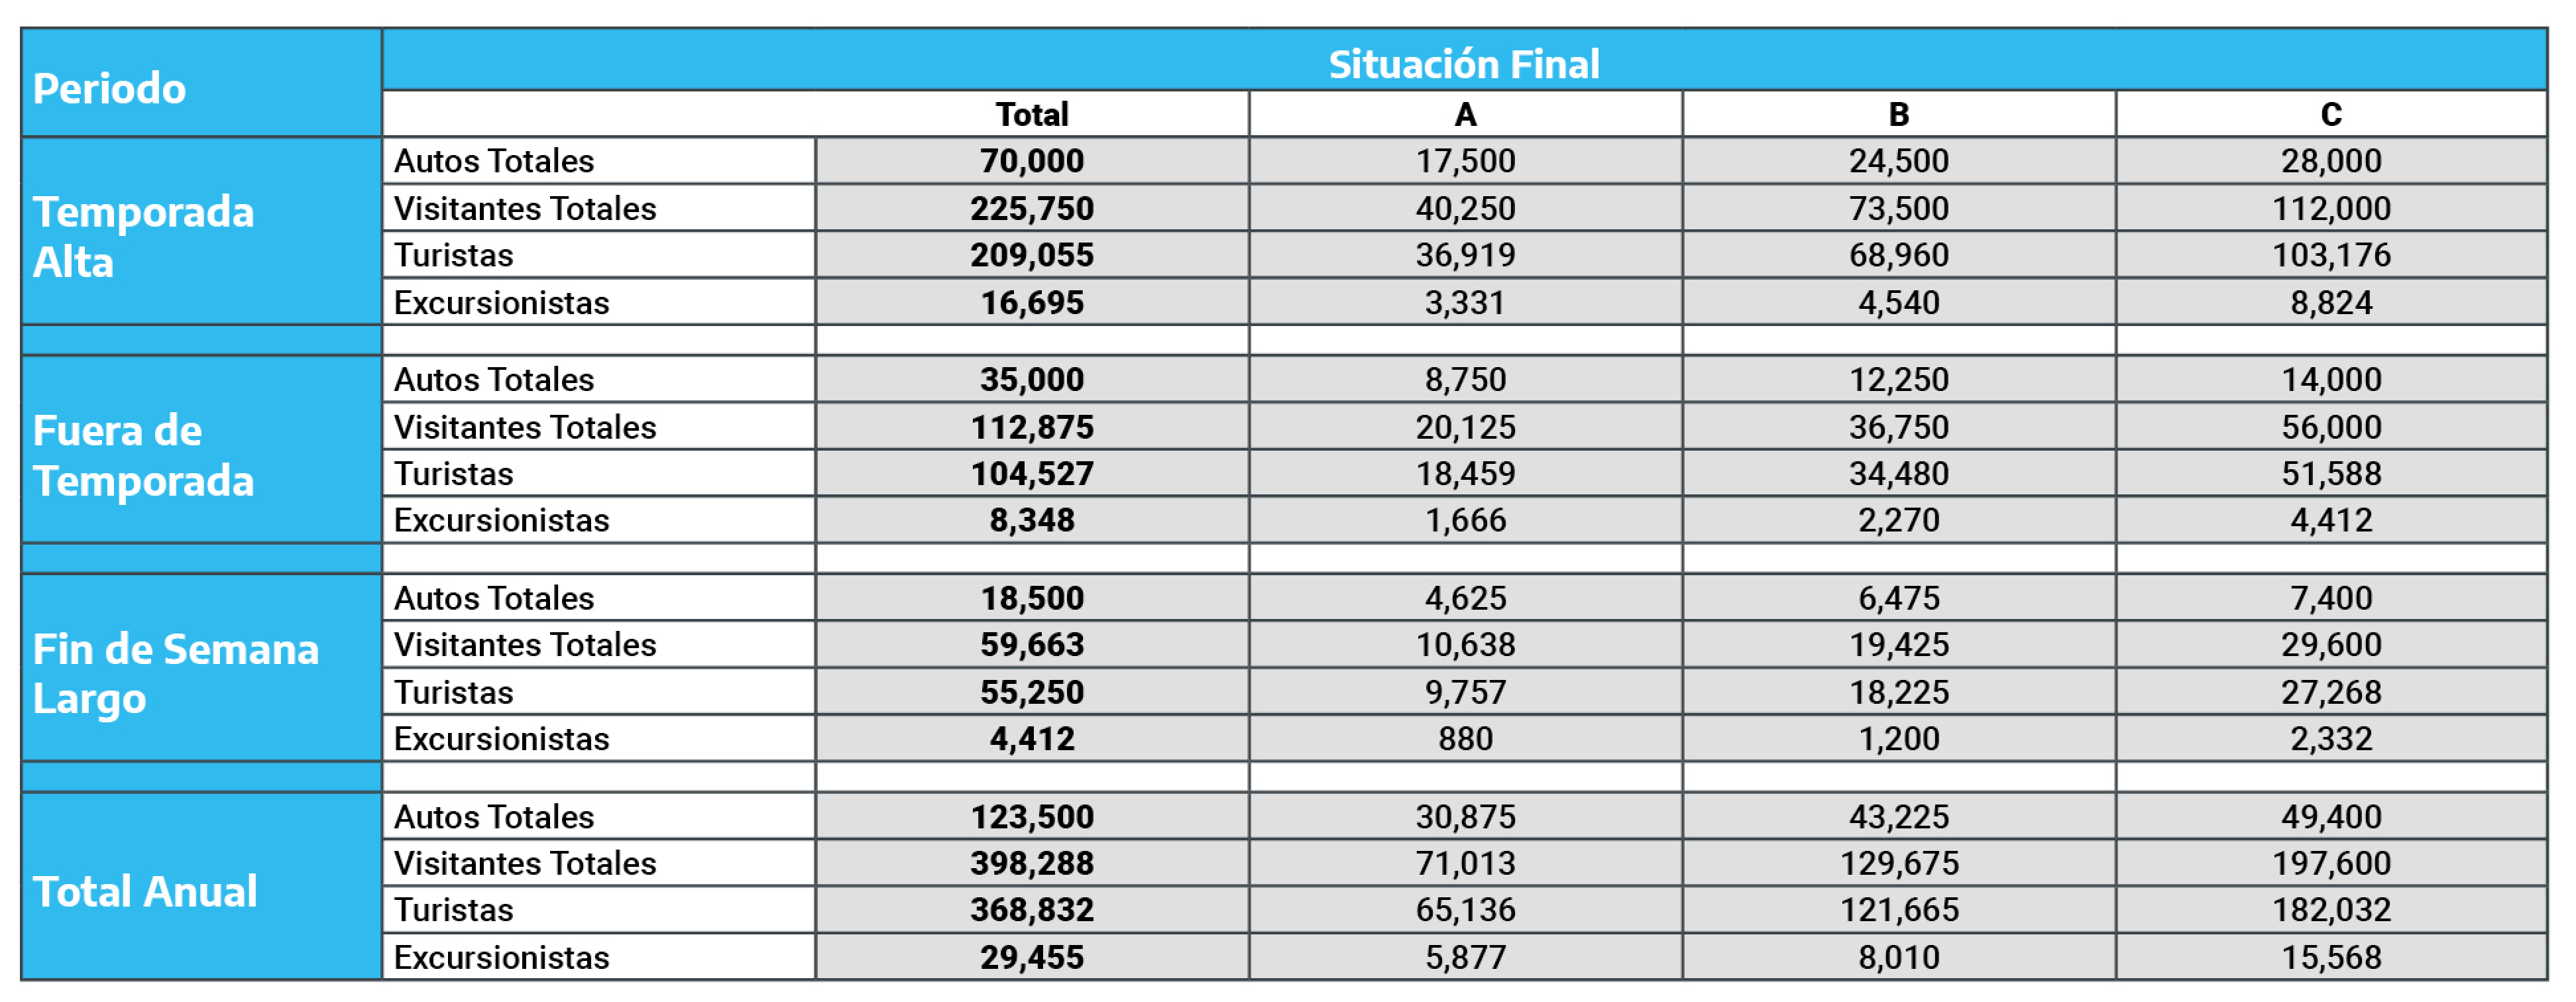
\includegraphics[width=1\linewidth]{imagenes/figura5B} 

}

\caption{Aplicación de coeficiente de Temporada Alta, obtenido del estudio realizado por la localidad C, a las cantidades de vehículos de todos los períodos (Temporada Alta, Fines de semana largo y Fuera de temporada)}\label{fig:temporadaalta}
\end{figure}

\hfill\break
Con estas dos Figuras se busca dar cuenta de la alteración que se produce en las estimaciones cuando no se toma en consideración la estacionalidad, mencionada en el primer capítulo. En este caso, si se aplica el coeficiente obtenido en temporada alta para todos los períodos, se estarían alterando las estimaciones de los períodos restantes. Por ejemplo, fuera de temporada, se sobreestimaría tanto los visitantes (en un \(25\%\)), como los turistas (en un \(54\%\)), mientras que los excursionistas sufrirían una subestimación del orden de un \(62,8\%\). Esto ocurre debido a que en temporada alta, es mayor la cantidad de visitantes y turistas en relación al total de vehículos que ingresan, y más común el ingreso de turistas en relación a los otros dos períodos. Análogas a las alteraciones descriptas para fuera de temporada alta se producen en el período de fines de semana(los excursionistas se hubieran visto reducidos en un \(-1,0\%\) y \(-78,4\%\), respectivamente, y sólo la cantidad de turistas hubiera crecido en un \(38,6\%\)).

Como conclusión de este ejemplo, es evidente que resulta fundamental la evaluación previa y la implementación de una metodología adecuada que permita realizar de la manera más fiel posible el proceso de conversión de los datos provistos por el \texttt{RA} (automóviles en el ejemplo) a unidades relevantes desde el punto de vista de la estadística del turismo (cantidad de visitantes -turistas y excursionistas- según localidad de destino en el ejemplo).

\hypertarget{terminales-de-pasajeros}{%
\section{Terminales de pasajeros}\label{terminales-de-pasajeros}}

\hfill\break
Las terminales de autobuses, aéreas y/o ferroviarias ofrecen una importante fuente de información secundaria a las instituciones generadoras de estadísticas de turismo de las provincias y los municipios ya que registran las cifras de ingresos y egresos de servicios (ómnibus, aviones y ferrocarriles). Dicho registro presenta una gran robustez por ser de tipo censal, es decir, se registran todos los servicios que ingresen o egresen de la provincia, departamento y/o municipio\footnote{Cabe señalar que esto puede no ser así en todos los casos. Por ejemplo, en las grandes ciudades suele ser común que en las terminales de ómnibus operen los servicios de ``larga distancia'' , mientras que los servicios regionales lo hacen desde otros puntos. En un caso como el planteado, si no se contempla esta situación y se asume que todos los visitantes que ingresan en ómnibus llegan a la terminal, se estaría subestimando el peso del turismo interno, es decir, de los visitantes que provienen de otros puntos de la provincia (siempre y cuando, obviamente, estos puntos se encuentren situados por fuera de lo que se ha postulado como distancia mínima en la definición del entorno habitual). Tampoco suelen operar en las terminales de ómnibus los servicios tipo chárter. En cambio, en las terminales áreas y acuáticas es difícil que se presente este tipo de situaciones.}.

Sin embargo, en general, estos \texttt{RA} no brindan información sobre los ingresos y egresos de personas, y, menos aún, si éstas resultan ser visitantes (turistas o excursionistas). En lo que a la identificación de visitantes y residentes corresponde, el dato sobre residencia juega un papel importante, ya que brinda una aproximación (los visitantes son un subtipo de viajero, determinado por haber salido de su entorno habitual).

Es en este último punto en el cual el procedimiento para la conversión de los datos suministrados por las terminales juega un rol fundamental. Si los datos son utilizados como indicadores en forma directa no sólo se estará perdiendo información sino que incluso se pueden extraer conclusiones erróneas: al tratarse de servicios públicos, la alteración en el flujo de ómnibus, trenes o aviones está sólo en parte sometida a variaciones de la demanda y, por otra parte, la proporción de residentes y visitantes en cada momento del año suele variar significativamente. Por tanto, es preciso implementar una estrategia metodológica adecuada para obtener información relevante desde el punto de vista de las estadísticas del turismo. En otras palabras, mientras que este tipo de \texttt{RA} brinda información desde el punto de vista de la oferta, sólo con un proceso de reconversión metodológica se podrá arribar a información sobre la demanda turística.

Siguiendo la línea de lo presentado anteriormente, en primer lugar se deberá definir la población objetivo, cuyo reconocimiento resulta fundamental como guía para los pasos subsiguientes del análisis. En este caso, la población objetivo serán los visitantes (turistas y excursionistas) que ingresen por alguna de las vías mencionadas (autobús, aérea o ferrocarril).

Una vez delimitada la población objetivo, se deben definir e identificar tanto las unidades que informará el \texttt{RA} en cuestión como los pasos requeridos para la obtención de la información estadística y su delimitación (tipo de servicio de transporte, alcance geográfico, periodos a considerar en el estudio, etc.).

A continuación se presenta, un ejemplo, como propuesta para el tratamiento y procesamiento de los datos provenientes de estas fuentes secundarias.

La localidad ``Norte'' posee un aeropuerto al que llegan tres vuelos diarios, los cuales cuentan con una capacidad total de 104 asientos por vuelo (312 diarios). Si bien se cuenta con una precisa contabilización de la oferta -llegadas y salidas- de servicios, se desconoce la cantidad de personas que ingresan, así como también la residencia de las mismas.

En primer lugar se deberá elaborar un coeficiente que permita determinar la cantidad de pasajeros que ingresan en los vuelos, y en segundo lugar, una distribución del lugar de residencia para poder clasificar a los pasajeros en ``visitantes'' y ``otros viajeros''\footnote{Toda persona que se desplace fuera de su entorno habitual por una duración mayor a doce meses o cuya finalidad primordial es ejercer una actividad remunerada en el lugar visitado. Dentro de este grupo se encuentran: emigrantes, trabajadores transfronterizos, viajeros en desplazamiento cotidiano al lugar de trabajo, diplomáticos y militares, refugiados, viajeros en tránsito.}, teniendo en consideración la definición de entorno habitual. Por tanto, se deberá realizar un operativo que permita determinar un coeficiente mediante el cual se logre estimar la cantidad de pasajeros y que proporción corresponde a cada uno de los grupos mencionados, distinguiendo a los visitantes entre turistas y excursionistas.

A fin de realizar el estudio propuesto y dotarlo de robustez, se han determinado, como en el ejemplo de la sección anterior, tres períodos de estudio: ``temporada alta'' , la cual posee una duración total de dos meses; ``fuera de temporada'' , la que alcanza en total los nueve meses; y ``fines de semana largo'' , los cuales sumados ascienden a 30 días, es decir un mes.

A continuación se calculan los asientos totales correspondiente a cada período en análisis, recordando que los tres vuelos diarios implicaban 312 asientos y simplificando la extensión de todos los meses a 30 días\footnote{En el ejemplo se asume que no se suspenderá ni agregará ningún vuelo a lo previsto. No obstante, si esto sucediera no sería ningún problema, pues solo habría que sustraer o adicionar asientos a la capacidad máxima disponible.}:

\begin{itemize}
\item
  Temporada alta: 18.720 asientos (312 asientos diarios*30días*2meses)
\item
  Fines de semana largo: 9.360 asientos (312 asientos diarios*30 días)
\item
  Fuera de temporada: 84.240 asientos (312 asientos diarios*30 días*9 meses)
\end{itemize}

Una vez determinada la capacidad máxima, se realiza un estudio que toma muestras independientes para cada período en análisis, a fin de poder dar cuenta de la heterogeneidad temporal de la afluencia turística al destino.

Además, estas muestras se construyen de maneras diversas, procurando que sean representativas de la variedad de situaciones al interior de cada periodo. En el caso de ``temporada alta'' y ``fuera de temporada'' , las mismas estarán conformadas por siete días distintos (lunes, martes, etc.) de semanas diferentes de cada una. Para los ``fines de semana largo'' la muestra comprende a cuatro días, también distintos, cada uno tomado de fines de semana largo con distintas características. Por tanto, debido a los datos mencionados anteriormente, se puede dar cuenta de los lugares totales que se contemplan en el estudio por temporada. Los mismos se enuncian a continuación:

\begin{itemize}
\item
  \textbf{Temporada alta:} 2.184 (312 asientos * 7 días)
\item
  \textbf{Fuera de temporada:} 2.184 (312 asientos * 7 días)
\item
  \textbf{Fines de semana largo:} 1.248 (312 asientos * 4 días)
\end{itemize}

\hfill\break
Se busca eliminar cualquier tipo de sesgo que se pueda generar por las grandes fluctuaciones que presenta el sector turístico (cuestiones económicas, climáticas, etc.). Es decir, por ejemplo, si se tomaran todos los días de una misma semana en la que se presentan condiciones meteorológicas muy desfavorables y eso se tomara como representativo de toda la semana, probablemente se distorsionaría el valor del coeficiente y, con ello, de la cantidad estimada a posteriori. En otro orden, si el estudio se realiza en semanas distintas, pero siempre el mismo día (por ejemplo, los sábados), también se podrían introducir sesgos si la demanda del destino presenta alguna particularidad bajo la cual en determinados días es más fuerte que en otros. Para evitar este tipo de distorsiones, los días en los que se realizará el estudio son seleccionados al azar (por sorteo) previamente.

El estudio contempla dos fases o dos tipos de relevamientos. Por un lado, se realiza un conteo de llegadas de pasajeros (esta tarea puede no ser necesaria, por ejemplo, si la empresa informa la cantidad de pasajeros embarcados); y por el otro, una pequeña encuesta a todos los pasajeros que arriban\footnote{En la práctica es casi imposible encuestar a todos los pasajeros en un estudio de este tipo, pues exige un enorme operativo de campo de muy corta duración, es decir, algo sumamente ineficiente. Para simplificar el razonamiento, aquí se postula que se encuesta a todos los que arriben en los vuelos estudiados. Debe considerarse que, en la práctica, los casos a encuestar deben ser seleccionados mediante un método que garantice la aleatoriedad, es decir, que no imponga un sesgo, como por ejemplo, encuestar a quienes ``parezcan extranjeros'' .} a fin de determinar si son residentes\footnote{Si bien este ejercicio apunta a cuantificar y caracterizar a los visitantes que llegan al destino, cabe notar que del mismo estudio podría surgir una estimación acerca del turismo emisivo, es decir, de los residentes en ese lugar que viajan a otros destinos.} o visitantes. En este último caso, se indaga sobre su lugar residencia (para diferenciar a los residentes en el país de quienes lo hacen en el exterior) y la duración prevista de la estadía (para clasificarlos en turistas o excursionistas).

Los resultados obtenidos son los que describen en la siguiente figura:

\begin{figure}

{\centering 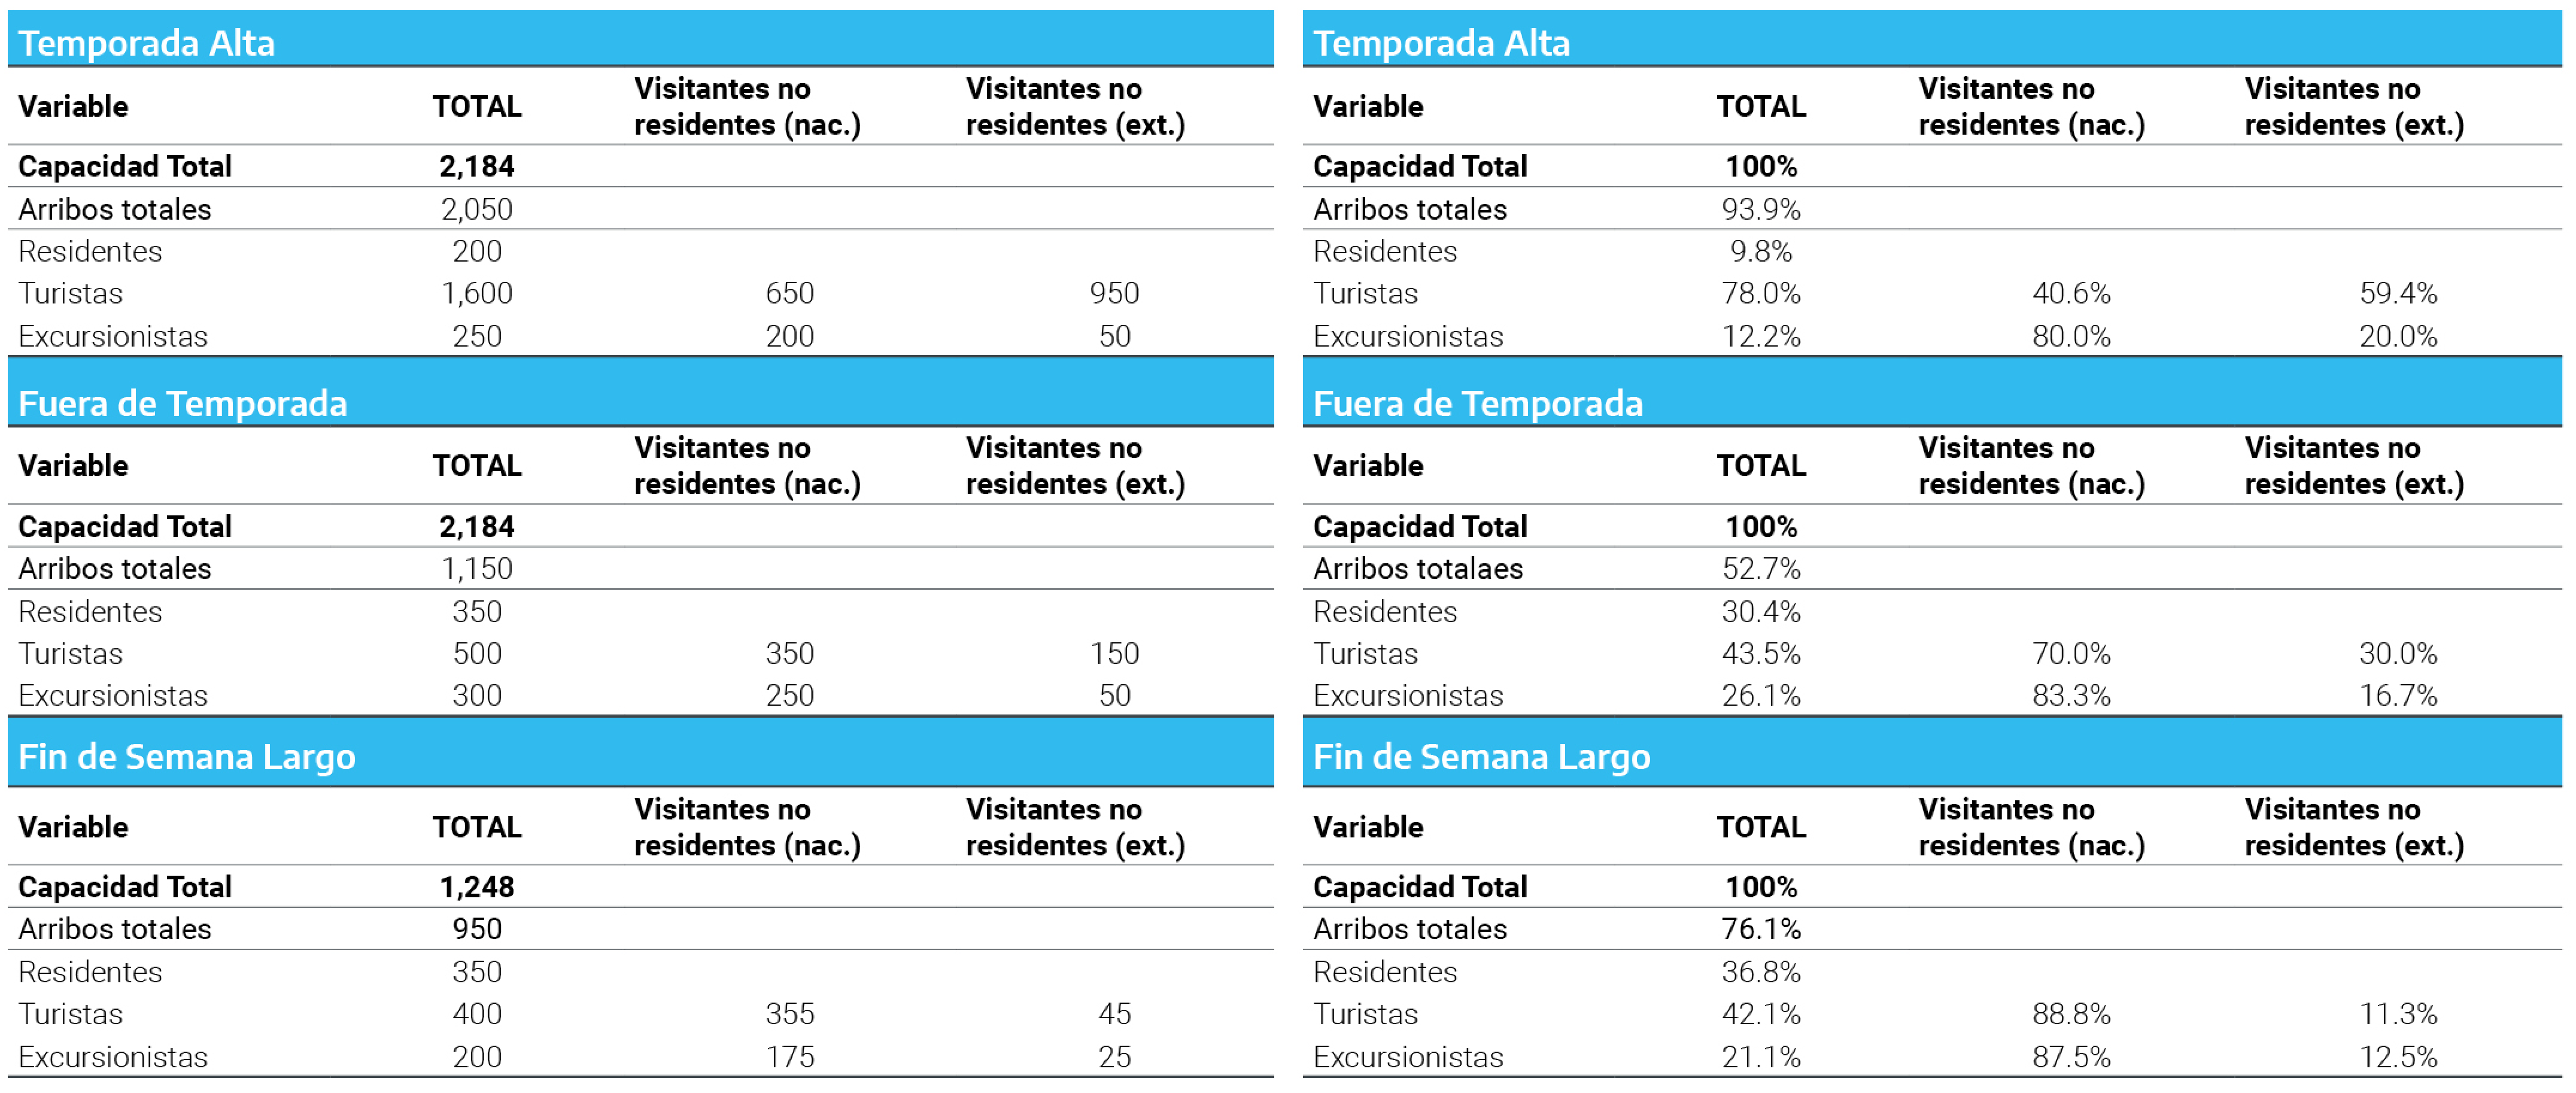
\includegraphics[width=1\linewidth]{imagenes/figura06} 

}

\caption{Resultados obtenidos por los estudios muestrales realizados por la localidad Norte}\label{fig:resultadosobtenidos}
\end{figure}

Si se encuesta a todas las personas que ingresen vía alguno de los aviones diarios se busca determinar, en primer lugar, el porcentaje de cantidad de llegadas sobre el total.

Si cada avión posee 104 asientos y diariamente hay tres llegadas, en los siete días contemplados para el estudio de temporada alta, la oferta de asientos (pasajes) alcanza a 2.184 asientos (104 x 3 x 7).

Si en el estudio realizado en 7 días de temporada alta se han contado un total de 2.050 llegadas de pasajeros, ello implica una tasa de ocupación del \(93,9\%\) sobre el máximo disponible (2.050 llegadas efectivas / 2.184 asientos disponibles).

Fuera de temporada los arribos alcanzaron un total de 1.150 pasajeros, lo que implica una ocupación del \(52,7\%\) del total de asientos disponibles.

Por último, en fines de semana largo, el relevamiento se realizó en 4 días (1.248 asientos) contándose 950 llegadas (\(76,1\%\) de ocupación de asientos).

Con estos resultados es posible estimar el total de pasajeros arribados al aeropuerto durante el año considerado, al aplicar la tasa de ocupación de cada periodo al total de asientos disponibles en cada uno de ellos.

La segunda fase es la aplicación de una encuesta muy simple a todos los pasajeros arribados para determinar, como se mencionó anteriormente, lugar de residencia y estadía en el destino (para el caso de los visitantes).

En el operativo realizado para temporada alta se da cuenta de que ingresaron un \(9,8\%\) de residentes y un \(90,2\%\) de visitantes (\(78\%\) de turistas y \(12,2\%\) de excursionistas). Un \(40,6\%\) de los turistas eran no residentes en Argentina y un \(59,4\%\) correspondieron a no residentes extranjeros; en el caso de los excursionistas, estas proporciones alcanzaron respectivamente al \(80\%\) y \(20\%\).

Para obtener los coeficientes correspondientes que cada categoría ocupa sobre la capacidad total, que servirá para realizar las estimaciones anuales, se presenta un ejemplo en el cuadro subsiguiente (Figura 3.5). En el mismo, se ejemplifica para temporada alta el caso de estimación de coeficientes de ``arribos de turistas no residentes (nac.)'' sobre la capacidad total. Los valores que deben ser multiplicados son provenientes de la Figura 3.4, es decir, del estudio realizado.

\begin{figure}

{\centering 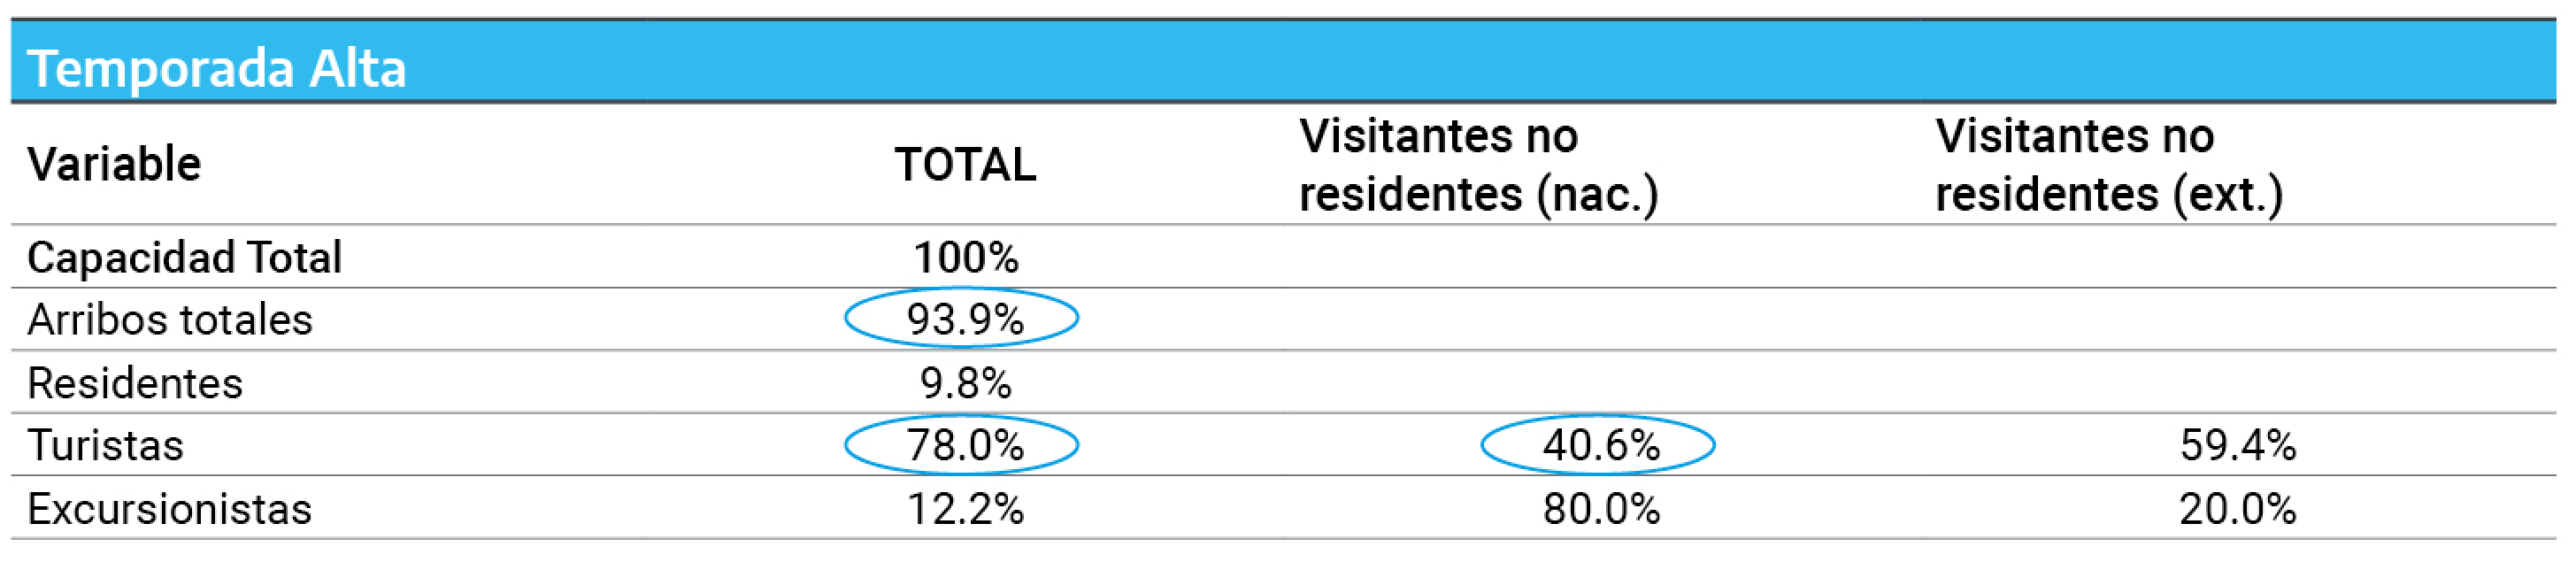
\includegraphics[width=1\linewidth]{imagenes/figura07} 

}

\caption{Estimación de coeficiente de arribos de turistas residentes sobre capacidad total}\label{fig:arribosdeturistas}
\end{figure}

Las estimaciones se obtienen a partir de multiplicar los porcentajes remarcados en la Figura 3.5 de la siguiente manera:\\

\begin{enumerate}
\def\labelenumi{\arabic{enumi}.}
\item
  Multiplicar el porcentaje de ``arribos totales'' con el de ``turistas'' (\(0,94\)*\(0,78\)=\(0,7332\)), para así obtener el peso de los turistas que han ingresado a la localidad ``Norte'' sobre el total de asientos disponibles (``capacidad total'').
\item
  Una vez obtenido dicho valor, se lo debe multiplicar por el porcentaje que corresponde a los ``visitantes no residentes (nac.)'' (esto es, el porcentaje de no residentes nacionales en total de turistas), a fin de obtener el peso de los turistas no residentes (nac.)que han ingresado sobre el total asientos o pasajes disponibles (\(0,7332\)*\(0,41\)=\(0,2976792\)). En efecto, se puede concluir que un \textbf{29,8\% de los asientos disponibles en los vuelos arribados durante la temporada alta han sido ocupados por turistas no residentes provenientes de otras localidades o provincias del país}.
\item
  Finalmente, para estimar la cantidad de visitantes en el periodo bajo estudio se debe multiplicar el coeficiente de cada celda por el total de asientos disponibles en el periodo. Si la temporada alta está comprendida por 2 meses, ello implica un total de 18.720 asientos disponibles. Si se estimó que el porcentaje de éstos ocupados por turistas no residentes alcanzaba al \(29,8\%\), ello implica una cantidad que alcanza a 5.567 turistas (\(0,298\)*\(18.720\)).
\end{enumerate}

El mismo cálculo debe ser realizado para los casos subsiguientes, de modo de poder estimar, a partir de los datos del \texttt{RA} y los coeficientes construidos, la cantidad de visitantes por tipo y lugar de residencia para el año entero.

En términos lógicos, sólo es preciso estimar, para cada periodo definido, el coeficiente que corresponde a cada una de estas cuatro categorías: (1) turistas no residentes nacionales, (2) turistas no residentes extranjeros, (3) excursionistas no residentes nacionales y (4) excursionistas no residentes extranjeros. La suma de las cuatro arroja un coeficiente que permite estimar el total de visitantes a partir de las plazas disponibles. La suma de 1 y 2, arroja el coeficiente del peso de los turistas (análogamente, 3+4= excursionistas) y la suma de 1 y 3 la de visitantes no residentes nacionales (análogamente, 2+4= visitantes no residentes extranjeros).

La Figura 3.6 da cuenta, en primer lugar, de los coeficientes para los grupos estratos de visitantes considerados por periodo (calculados como en el ejemplo de la Figura 3.5); luego, aplicando estos valores sobre la cantidad de asientos disponibles (capacidad total) en cada periodo, se obtienen las cantidades de visitantes correspondientes por categoría. Por ejemplo, si para la temporada alta, la llegada de turistas no residentes nacionales ocupó un \(29,8\%\), ese porcentaje es multiplicado por la capacidad total de asientos en dicho período (en este caso: 18.720), para así obtener la cantidad estimada de llegadas en un año durante la temporada alta.

\begin{figure}

{\centering 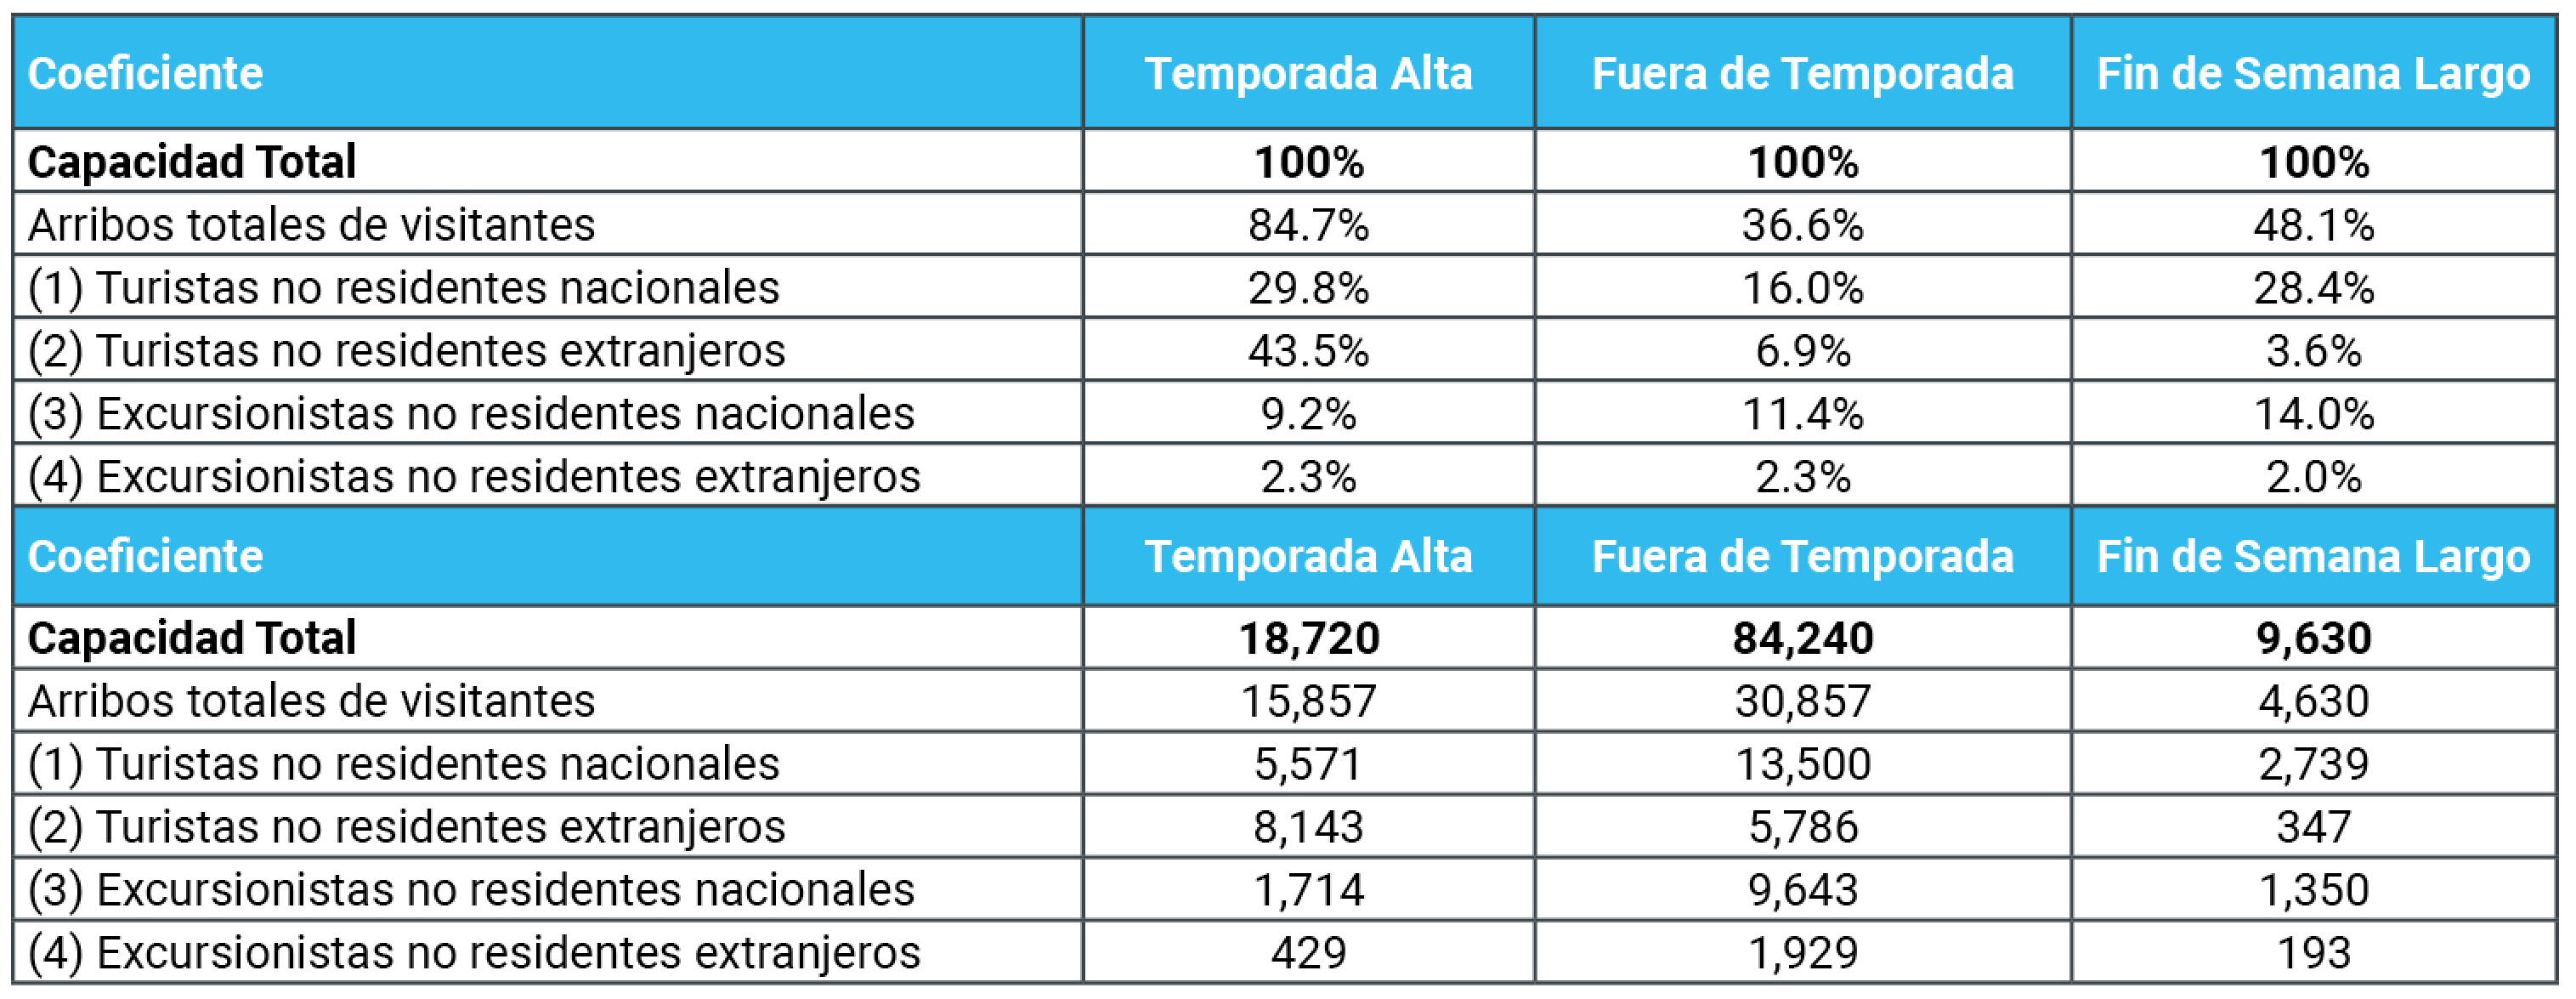
\includegraphics[width=1\linewidth]{imagenes/figura08} 

}

\caption{Estimación de llegadas por tipo y residencia de visitante en cada período bajo estudio}\label{fig:llegadasportipo}
\end{figure}

Es importante remarcar el hecho de que los coeficientes varían en forma significativa en cada uno de los períodos tomados en consideración. Como en el ejemplo anterior, de haberse aplicado un coeficiente único que no contemple las fluctuaciones estacionales, se hubiese perdido muchísima información y se hubieran introducido sesgos que, posiblemente, invalidarían las estimaciones.

Por otro lado, debido a la variabilidad que caracteriza a la demanda turística, se debe tener en cuenta que los resultados obtenidos deberán ser actualizados cada cierto tiempo a fin de reflejar del modo más fehaciente la realidad del sector. Si es preciso realizar un estudio para el cálculo de los coeficientes de conversión todos los años, cada tres o cada cinco años, etc., dependerá de las características del destino, del nivel de estabilidad de la demanda, del grado de precisión buscado, de los objetivo finales para los cuales se procura obtener la información, etc.

\hypertarget{centro-de-informaciuxf3n}{%
\section{Centro de Información}\label{centro-de-informaciuxf3n}}

Tomando en consideración a otro de los \texttt{RA} que permite construir datos que den cuenta de la Demanda Turística, como ser los registros de llegadas a los CIT, el procedimiento de utilización que se propone es el siguiente.

En primer lugar, identificar a la población objetivo: los visitantes (tanto turistas como excursionistas) que vayan a solicitar información a los CIT\footnote{Es decir, no será el universo de visitantes en la provincia, departamento y/o municipio lo que se estará estudiando, sino un subconjunto de éstos. Por otro lado, no es poco usual que residentes en un destino se acerquen a un CIT en búsqueda de información. No obstante tal situación no se contempla aquí para no complejizar el ejemplo.\\
}. Luego, se deberá determinar el alcance geográfico (provincia, municipio, etc.) y temporal del estudio.

Seguidamente se presenta un ejemplo propuesto siguiendo los pasos mencionados. En la localidad ``X'' se posee un único CIT que funciona en temporada alta (3 meses) y registra en forma diaria la cantidad de individuos que ingresan a consultar información (``consultas atendidas'').

Para poder obtener a partir de este dato información sobre el total de visitantes, y su distribución por tipo y residencia, se realiza un relevamiento especial en 15 días sorteados al azar (cuidando las proporciones entre días hábiles y no hábiles) indagando a todos los que ingresen en esos días por las siguientes variables:

\begin{itemize}
\item
  \textbf{Cantidad de individuos} que ingresan en busca de información.
\item
  \textbf{Cantidad de ingresos totales}: corresponde a la suma de los integrantes de los grupos de viaje de quienes se acercan a buscar información.
\item
  \textbf{Origen}: residentes de otra localidad de la provincia/argentinos de otras provincias/extranjeros.
\item
  \textbf{Tipo de visitante}: turista, excursionista o excursionista que es turista en otro destino\footnote{Esta categoría hace referencia a aquellos visitantes que se encuentran realizando un viaje multidestino como turistas, pero que visitan a la localidad en calidad de excursionistas. Es decir, si bien pernoctan fuera de su entorno habitual, no lo hacen en la localidad que se encuentra bajo estudio, en la cual se quedan menos de un día.}.
\end{itemize}

Los resultados informados son los que se exponen a continuación, en la Figura 3.7

\begin{figure}

{\centering 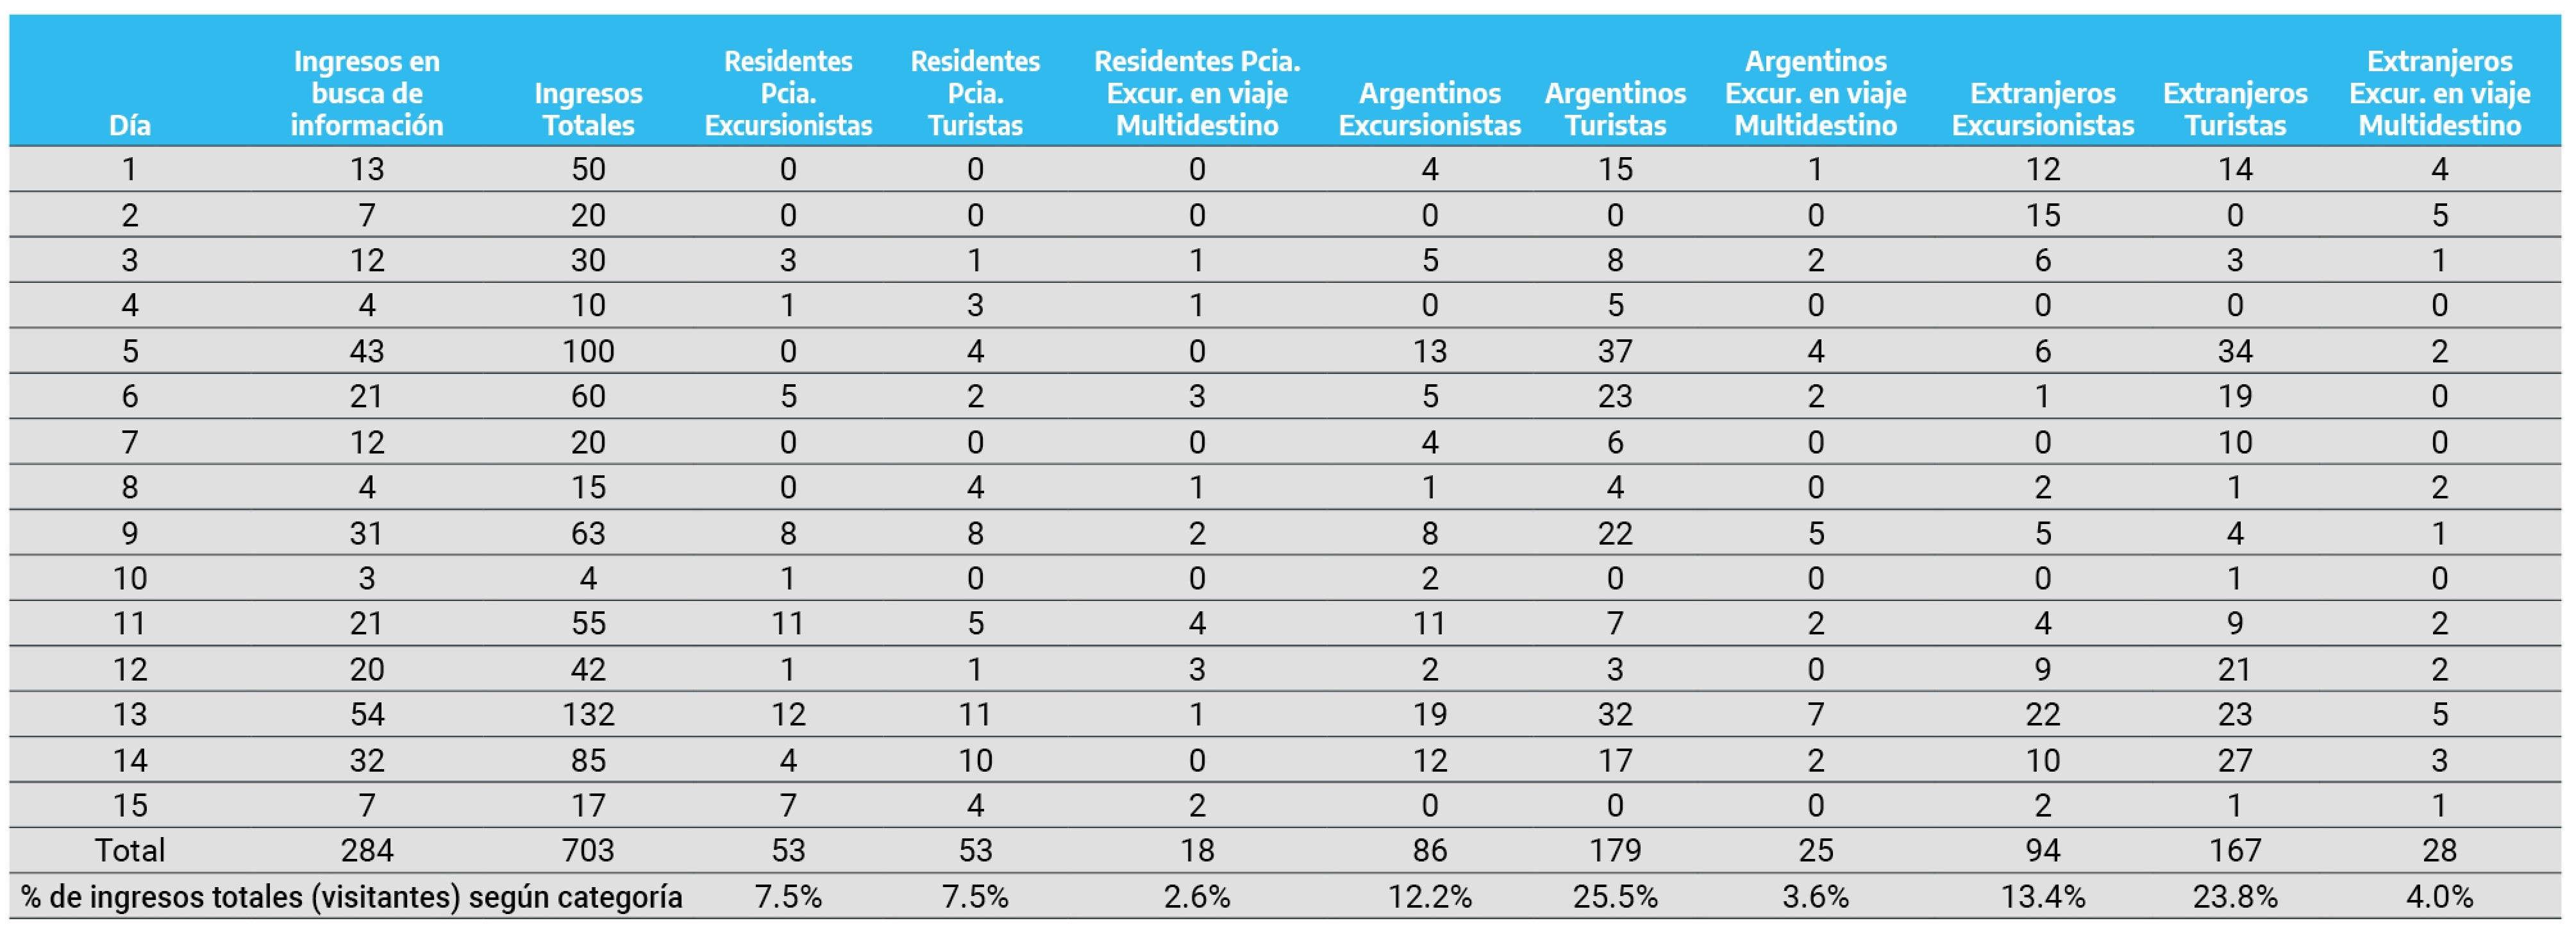
\includegraphics[width=1\linewidth]{imagenes/figura09} 

}

\caption{Cantidad de visitantes por categoría informados por el CIT y cálculo de porcentaje que los mismos ocupan sobre el total de ingresos}\label{fig:cantidaddevisitantes}
\end{figure}

Con los datos relevados, el instituto generador de estadísticas de la localidad procede a determinar el porcentaje de visitantes que ingresan en busca de información al CIT según categoría. En el caso de los excursionistas, un \(7,54\%\) son residentes de otras localidades de la provincia, un \(12,2\%\) nacionales y un \(13,4\%\) extranjeros. Entre los turistas que ingresaron al CIT se cuenta con un \(7,5\%\), un \(25,5\%\) y un \(23,8\%\), respectivamente. Por último, aquellos excursionistas que son turistas en un viaje multidestino, un \(2,6\%\) de éstos pertenecen a otras localidades de la misma provincia, un \(3,6\%\) a otras provincias del país y un \(4,0\%\) a otros países.

Resulta relevante destacar que estos porcentajes han sido calculados sobre el total de visitantes (suma de integrantes de los grupos de viajes que, mediante uno de sus componentes, se dirigieron al CIT), y no de los ingresos al CIT de las personas, consideradas individualmente, que en busca de información, a fin de poseer una visión con mayor exactitud sobre la realidad del sector turístico.

A partir de los datos sobre cantidad de consultas atendidas y de los coeficientes obtenidos en el estudio ad hoc, se podrá estimar las cantidades de visitantes de cada categoría que ingresan a los CIT en el total de la temporada.

Como ya se mencionó en ejemplos anteriores, se debe tener en consideración que cuando se elaboran coeficientes de estimación, éstos deben ser actualizados cada cierto período de tiempo y modificados a raíz del componente estacional que el sector turístico presenta. Es decir, se deberá contar con distintos coeficientes para cada tipo de momento turístico, por ejemplo: uno para ``temporada alta'' y otro para ``temporada baja''; así como también, actualizar éstos cada dos o tres años a fin de reflejar la variabilidad que se puede presentar en la afluencia turística. En el caso de que los coeficientes se mantengan constantes, sólo podría serlo producto de que mediante sucesivas instancias de testeo no se generen variaciones que requieran modificaciones de éstos.

Por otra parte, si la localidad en cuestión cuenta con una encuesta de perfil dirigida a los visitantes, en la misma se puede agregar una pregunta a fin de indagar si éstos han concurrido o no en busca de información a los CIT.

Así, si del estudio se desprende que durante la temporada surge que hubo 1.500 visitantes que pasaron (ellos u otros integrantes de su grupo) por el CIT y en otra encuesta surge que el 25\% de los visitantes concurrieron al CIT es posible estimar el volumen total de visitantes en la temporada, mediante una sencilla regla de tres simple: si los 1.500 visitantes que pasaron por CIT representan al \(25\%\) de los visitantes de un destino, el total de visitantes al mismo fue de 6.000.

Más allá de este ejemplo, la cobertura de este tipo de \texttt{RA} puede variar de destino y destino, y conviene siempre tener presente la población objetivo que se está estudiando. Es decir, no sólo no es posible con los datos obtenidos de este \texttt{RA} y el procedimiento ad hoc estimar la cantidad total de visitantes que ingresaron a la localidad ``X'' durante cierto período, sino que tampoco se podrán hacer generalizaciones (más allá del propio universo de visitantes al CIT) sobre sus características, por ejemplo: el tipo de visitante o, el lugar de residencia, que muy probablemente diferirán entre los visitantes que pasan por el CIT y los que no lo hacen.

A su vez, si bien el relevamiento se ejecuta en forma diaria, realizar un estudio con esa frecuencia no tendría sentido en términos estadísticos (la estadística sugiere períodos de análisis); por lo tanto sería pertinente determinar el período de análisis (semanal, quincenal, mensual, etc.). Incluso, ante fines de semana largos y/o semanas festivas significativas en términos turísticos para dicha localidad que merezca relevancia de ser estudiada.

Asimismo, para la cuantificación de otras variables como son la cantidad de pernoctes, el gasto realizado (sea diario, promedio, total, etc.), lugares visitados, etc. se deberá contar con la información desagregada al igual que el tipo de nacionalidad, para que, posteriormente se puedan elaborar estadísticas similares. Es decir, si el CIT cuenta con una encuesta, se deberán agregar preguntas que indaguen sobre dichas cuestiones a fin de poder estudiarlas tal como en el caso ejemplificado.

Por otro lado, en el caso en que no se pueda llevar a cabo, en forma continua, una encuesta que indague sobre las variables mencionadas anteriormente, se deberá estudiar la posibilidad de implementar un operativo alternativo que permita estimarlas. Uno de ellos es ejecutar una encuesta, dentro del CIT, en determinados períodos muestrales a fin de poder calcular coeficientes y/o fórmulas que permitan estimar dichas dimensiones\footnote{Para mayor detalle ver ejemplo de la sección Terminales de Pasajeros (Ómnibus, Aéreas y/o Ferroviarias)}. Éste sería un método correcto de estimación, pero se deben tener en cuenta algunas aclaraciones y/o recomendaciones metodológicas para proceder.\\
~\\
~\\
~\\

\hypertarget{bibliografuxeda}{%
\chapter*{\texorpdfstring{\textbf{Bibliografía}}{Bibliografía}}\label{bibliografuxeda}}
\addcontentsline{toc}{chapter}{\textbf{Bibliografía}}

  \bibliography{book.bib,packages.bib}

\end{document}
